For each data file (0...4), the absolute value of the combined receiver spectrum versus doppler frequency and range is shown as a colorplot for each of the two methods.

Also, for each data file, the spectrum of range gate number 35 is shown (combined receivers) together with both of the fittings from \inlinecodee{scipy.optimize.curve\_fit} and the method of moments.\\

A lot of these plots have missing parameter values along the range for those ranges where no fit could be determined due some issue with NaN values in the width calculation using the method of moments. \\

There are some with outlier values of the doppler shift. An analysis of the amplitude/power values at these points shows that the amplitude / SNR is too low for them to be considered as a correct result. In any case, one has to look at the combination of each of the graphs to make sense of them and judge whether a result is suitable for further considerations.\\

Comparing both methods, one finds that usually both follow a similar trajectory. Juding from the single-range-gate figures, the curve fitting approach seems to be more accurately estimating the doppler shift and amplitude. But the attractiveness of the moments-method might lie in the simplistic calculation approach which might yield better performance.

\subsection{File 1}
\begin{figure}[H]
  \begin{minipage}[t]{0.45\textwidth}
    \centering
    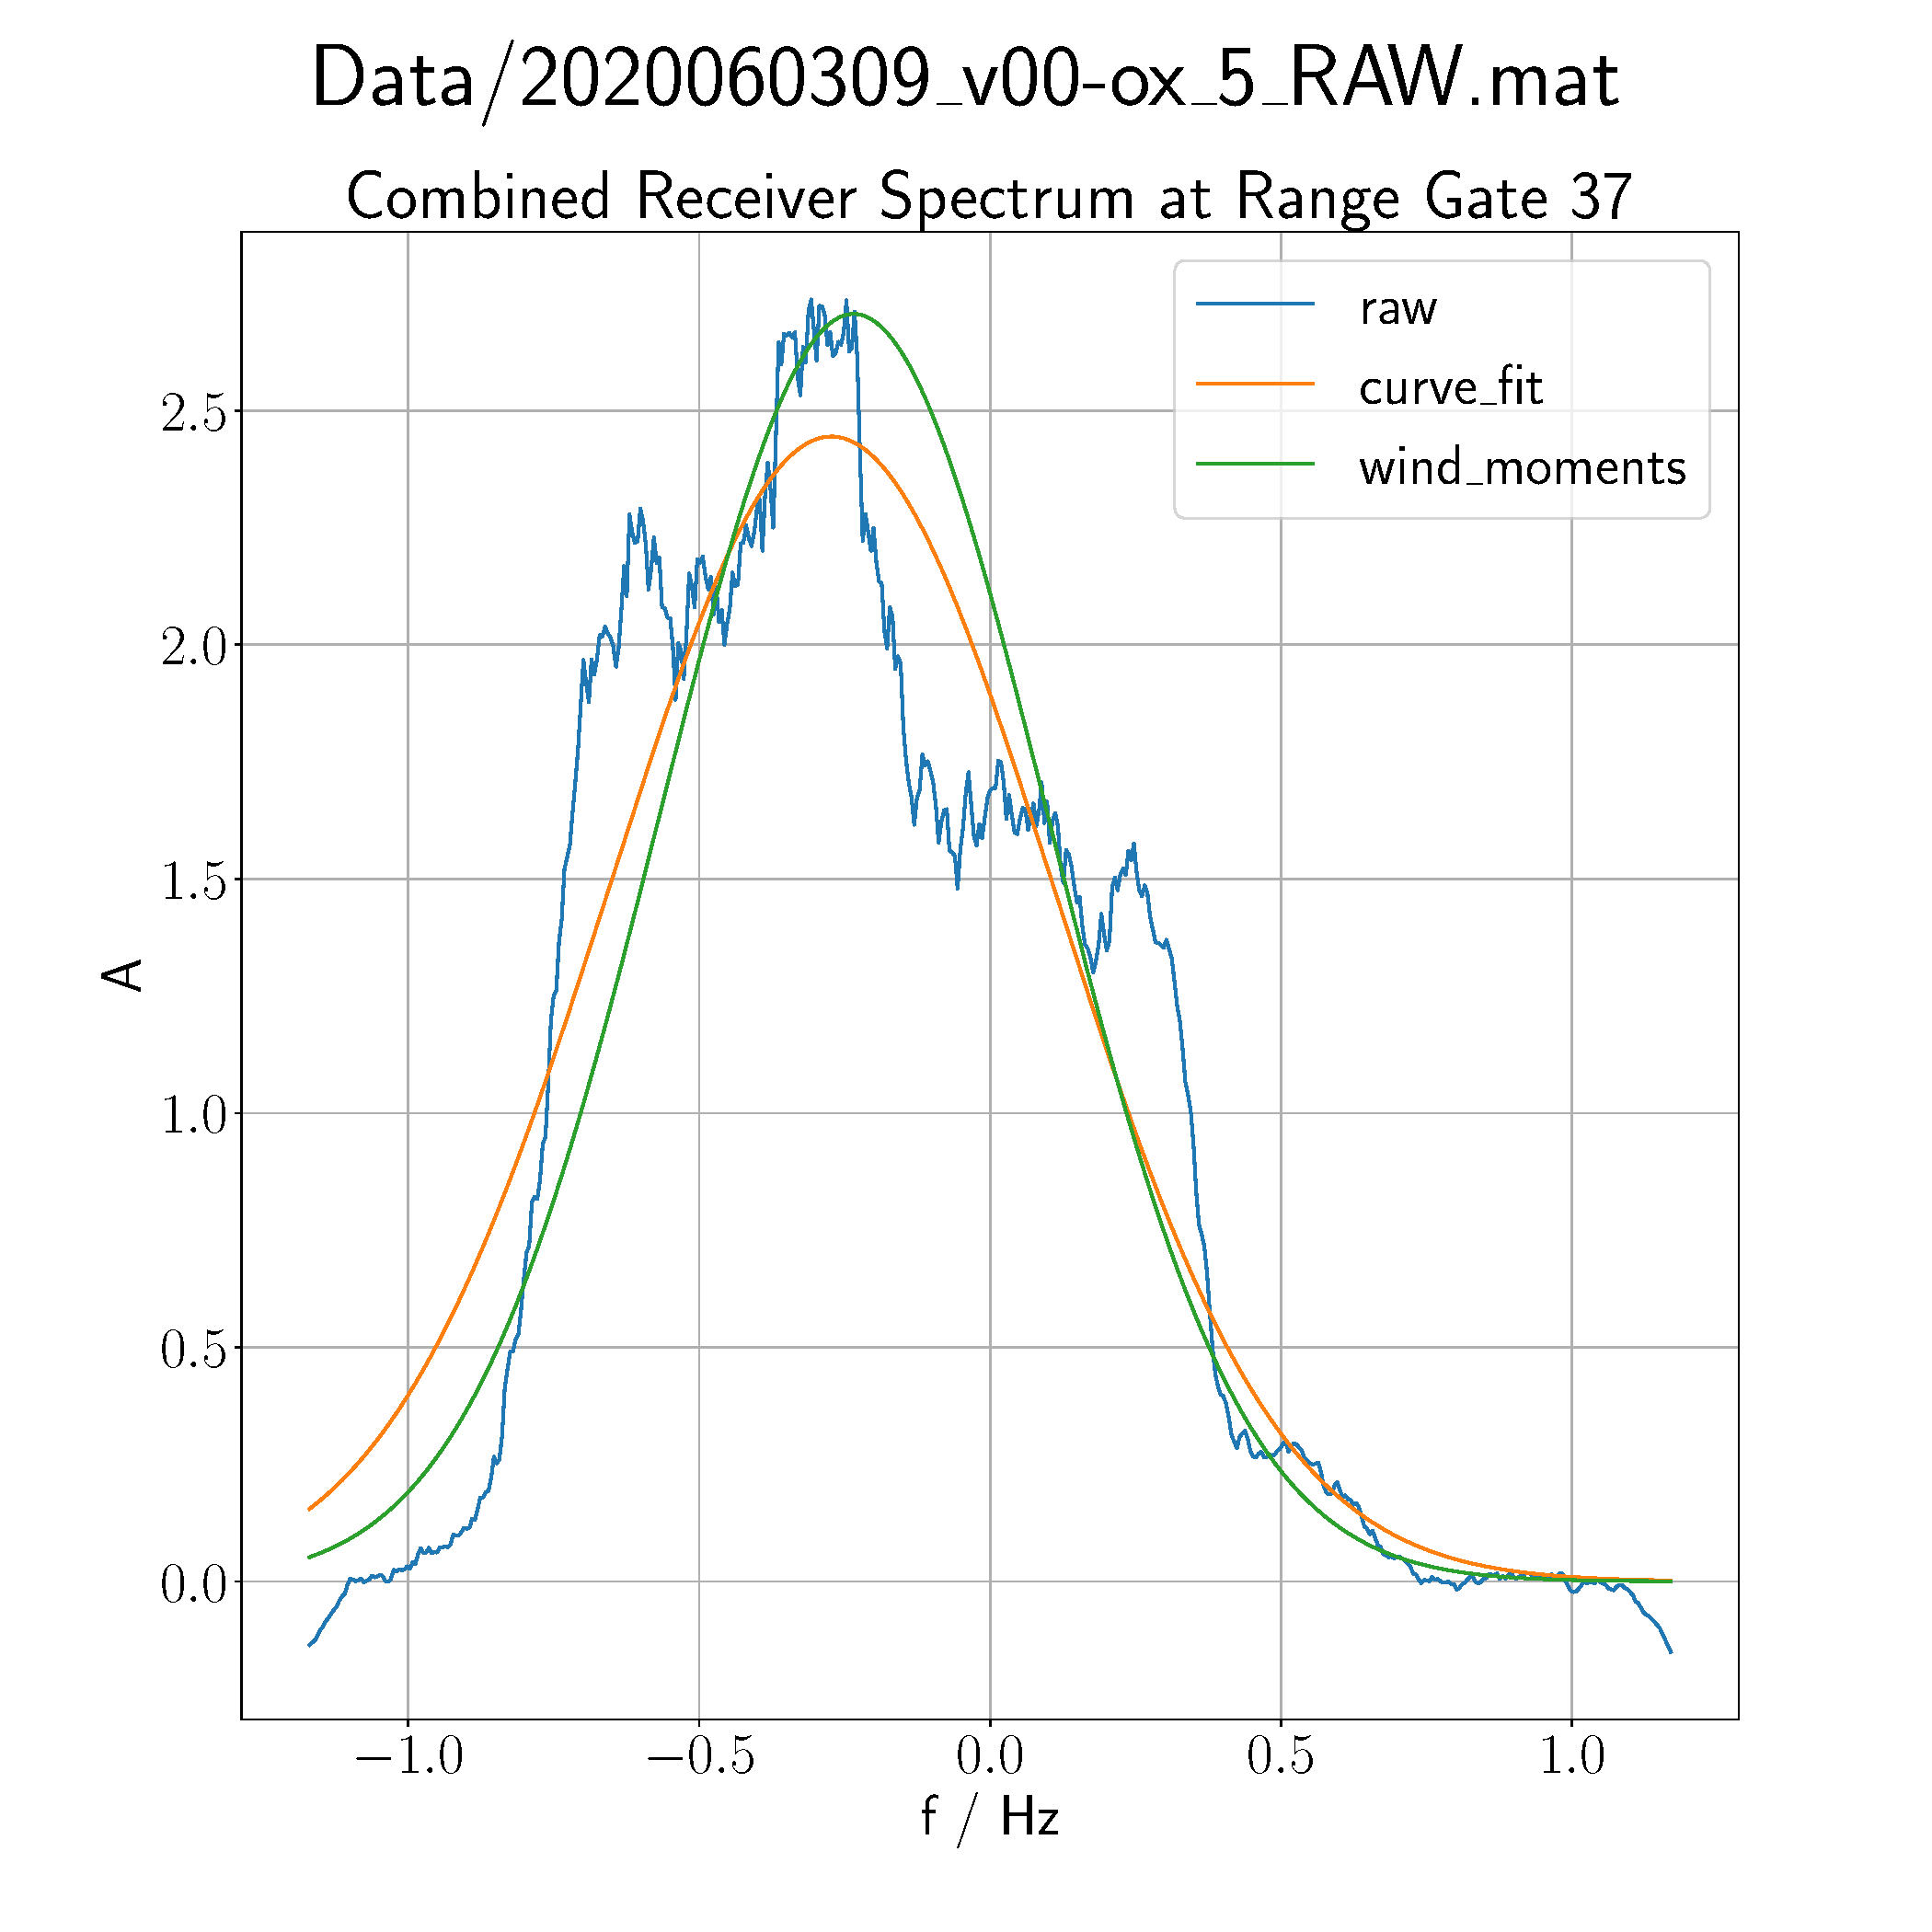
\includegraphics[width=\textwidth]{graphics/data_0_single_rg.pdf}
    \caption{}
  \end{minipage}\hfill
  \begin{minipage}[t]{0.45\textwidth}
    \centering
    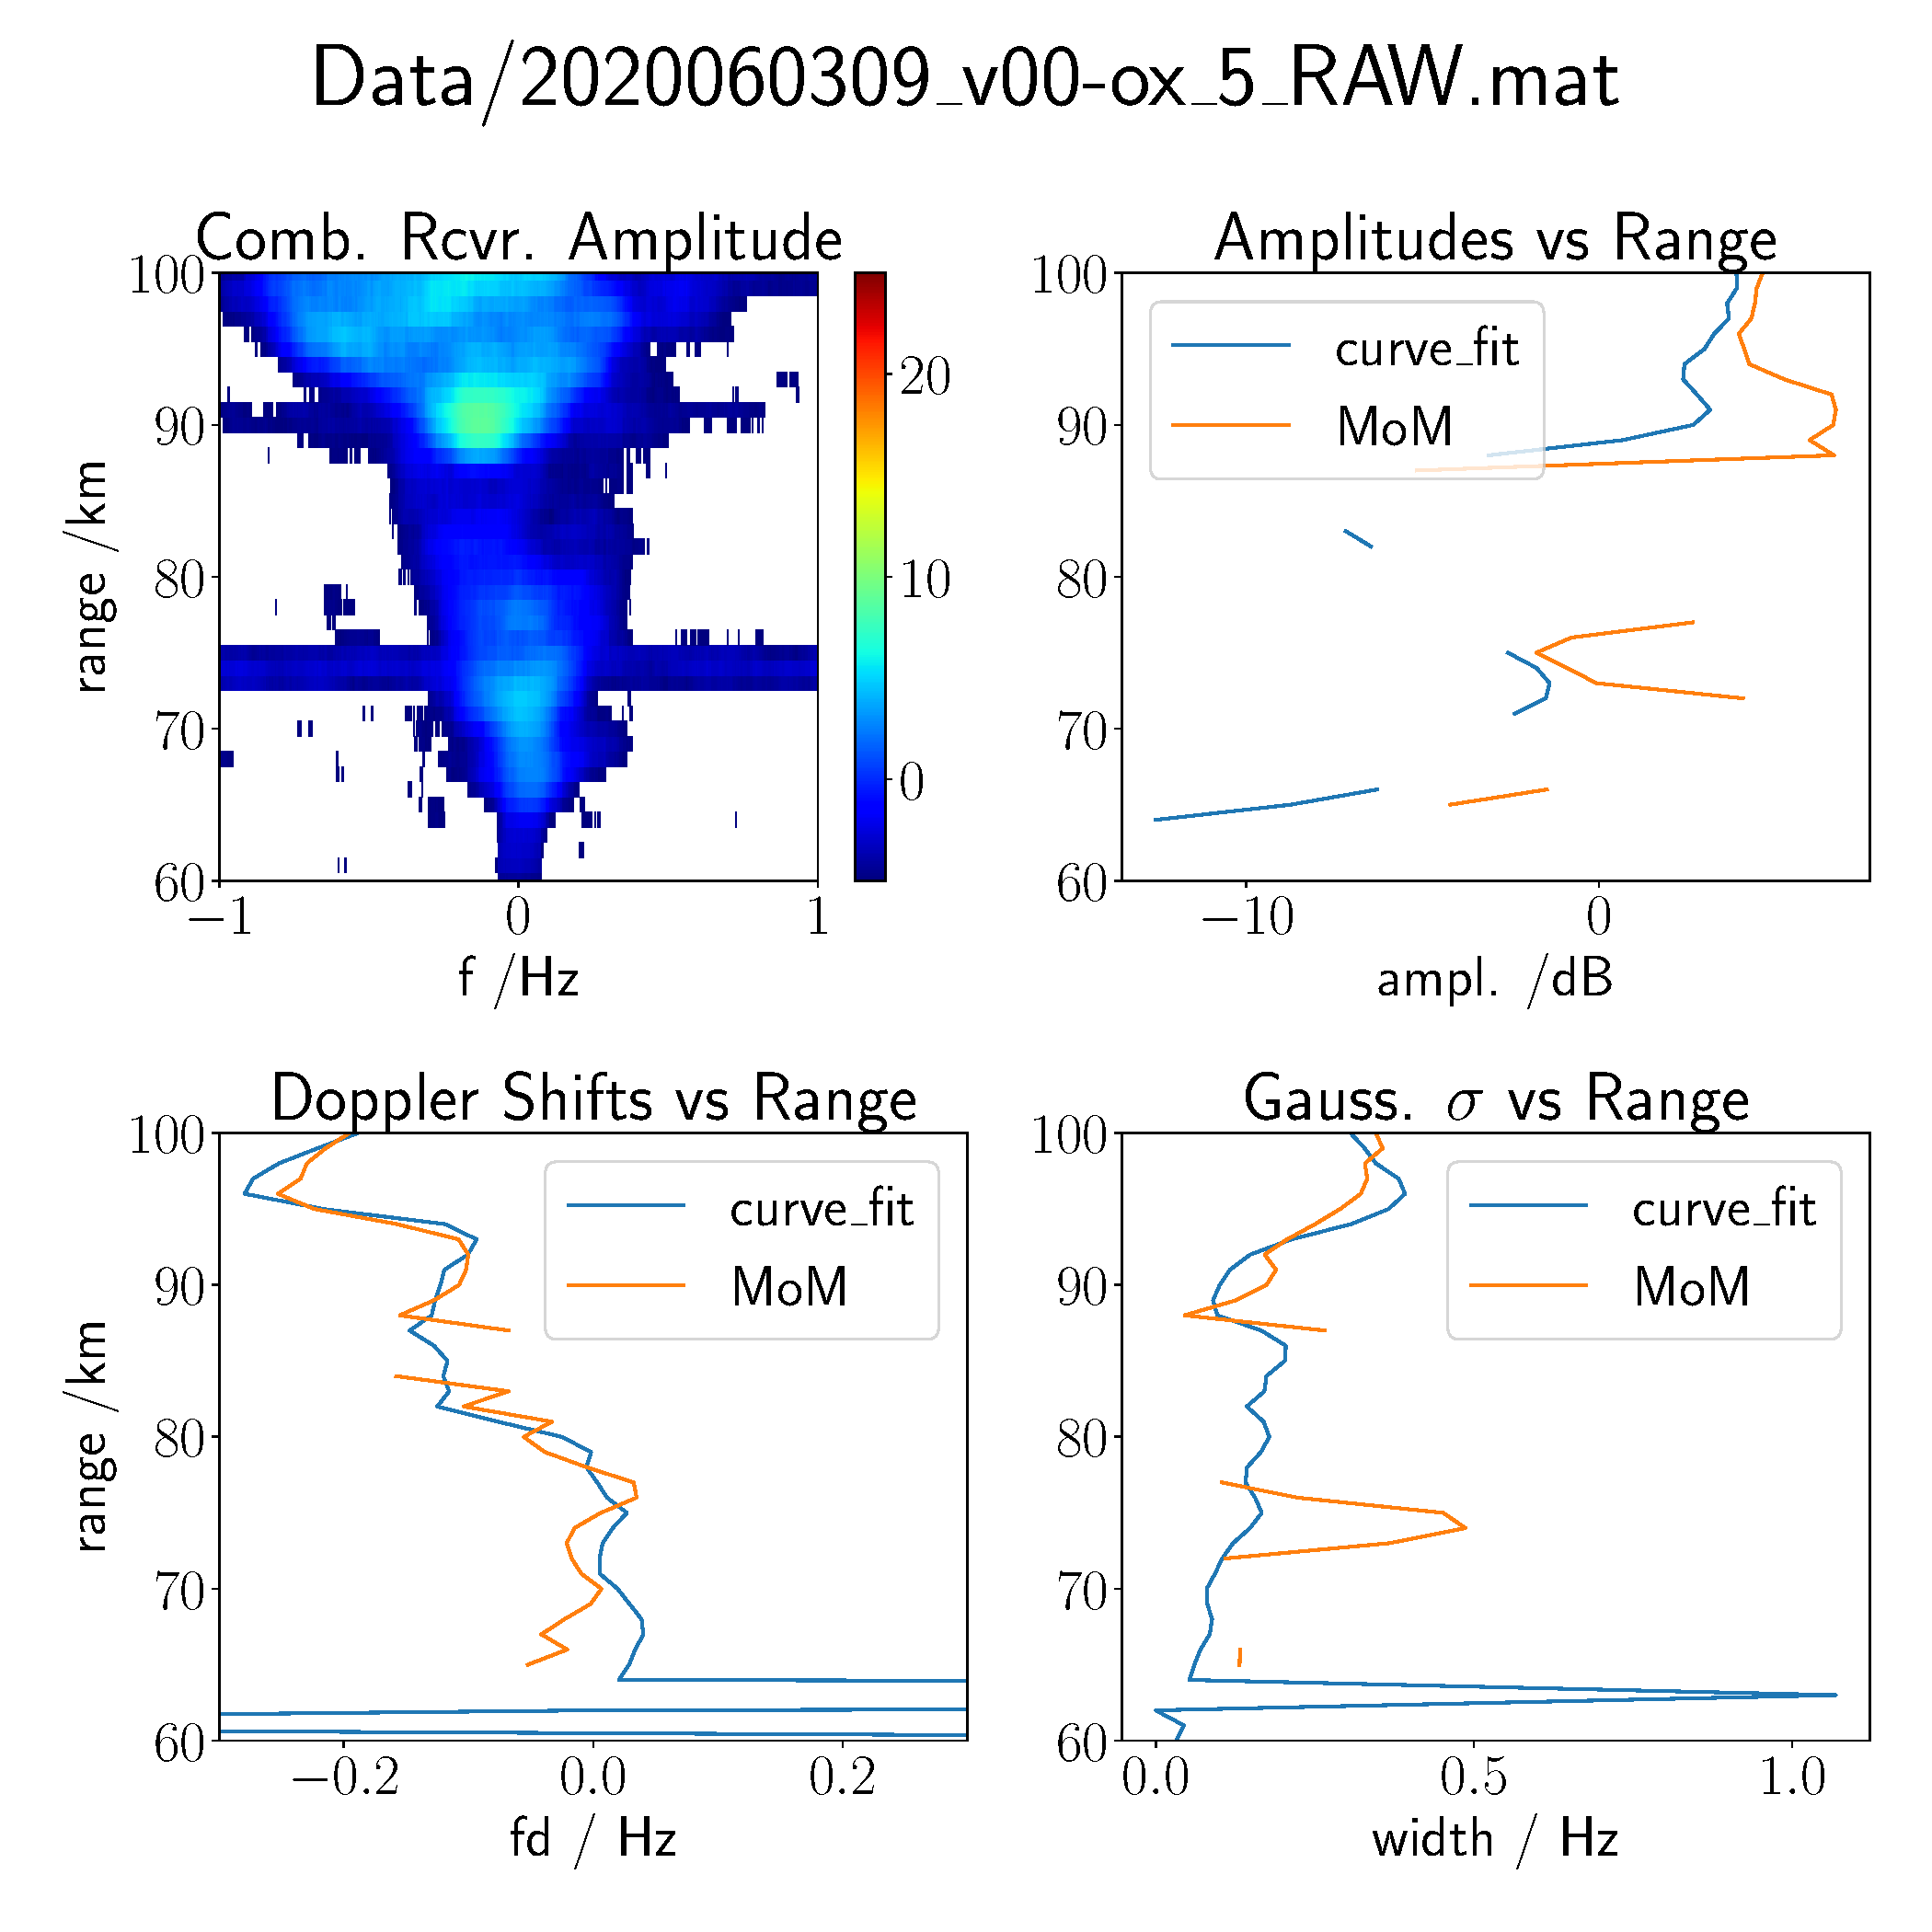
\includegraphics[width=\textwidth]{graphics/data_0_quad.pdf}
    \caption{}
   \end{minipage}
\end{figure}


\subsection{File 2}
\begin{figure}[H]
  \begin{minipage}[t]{0.45\textwidth}
    \centering
    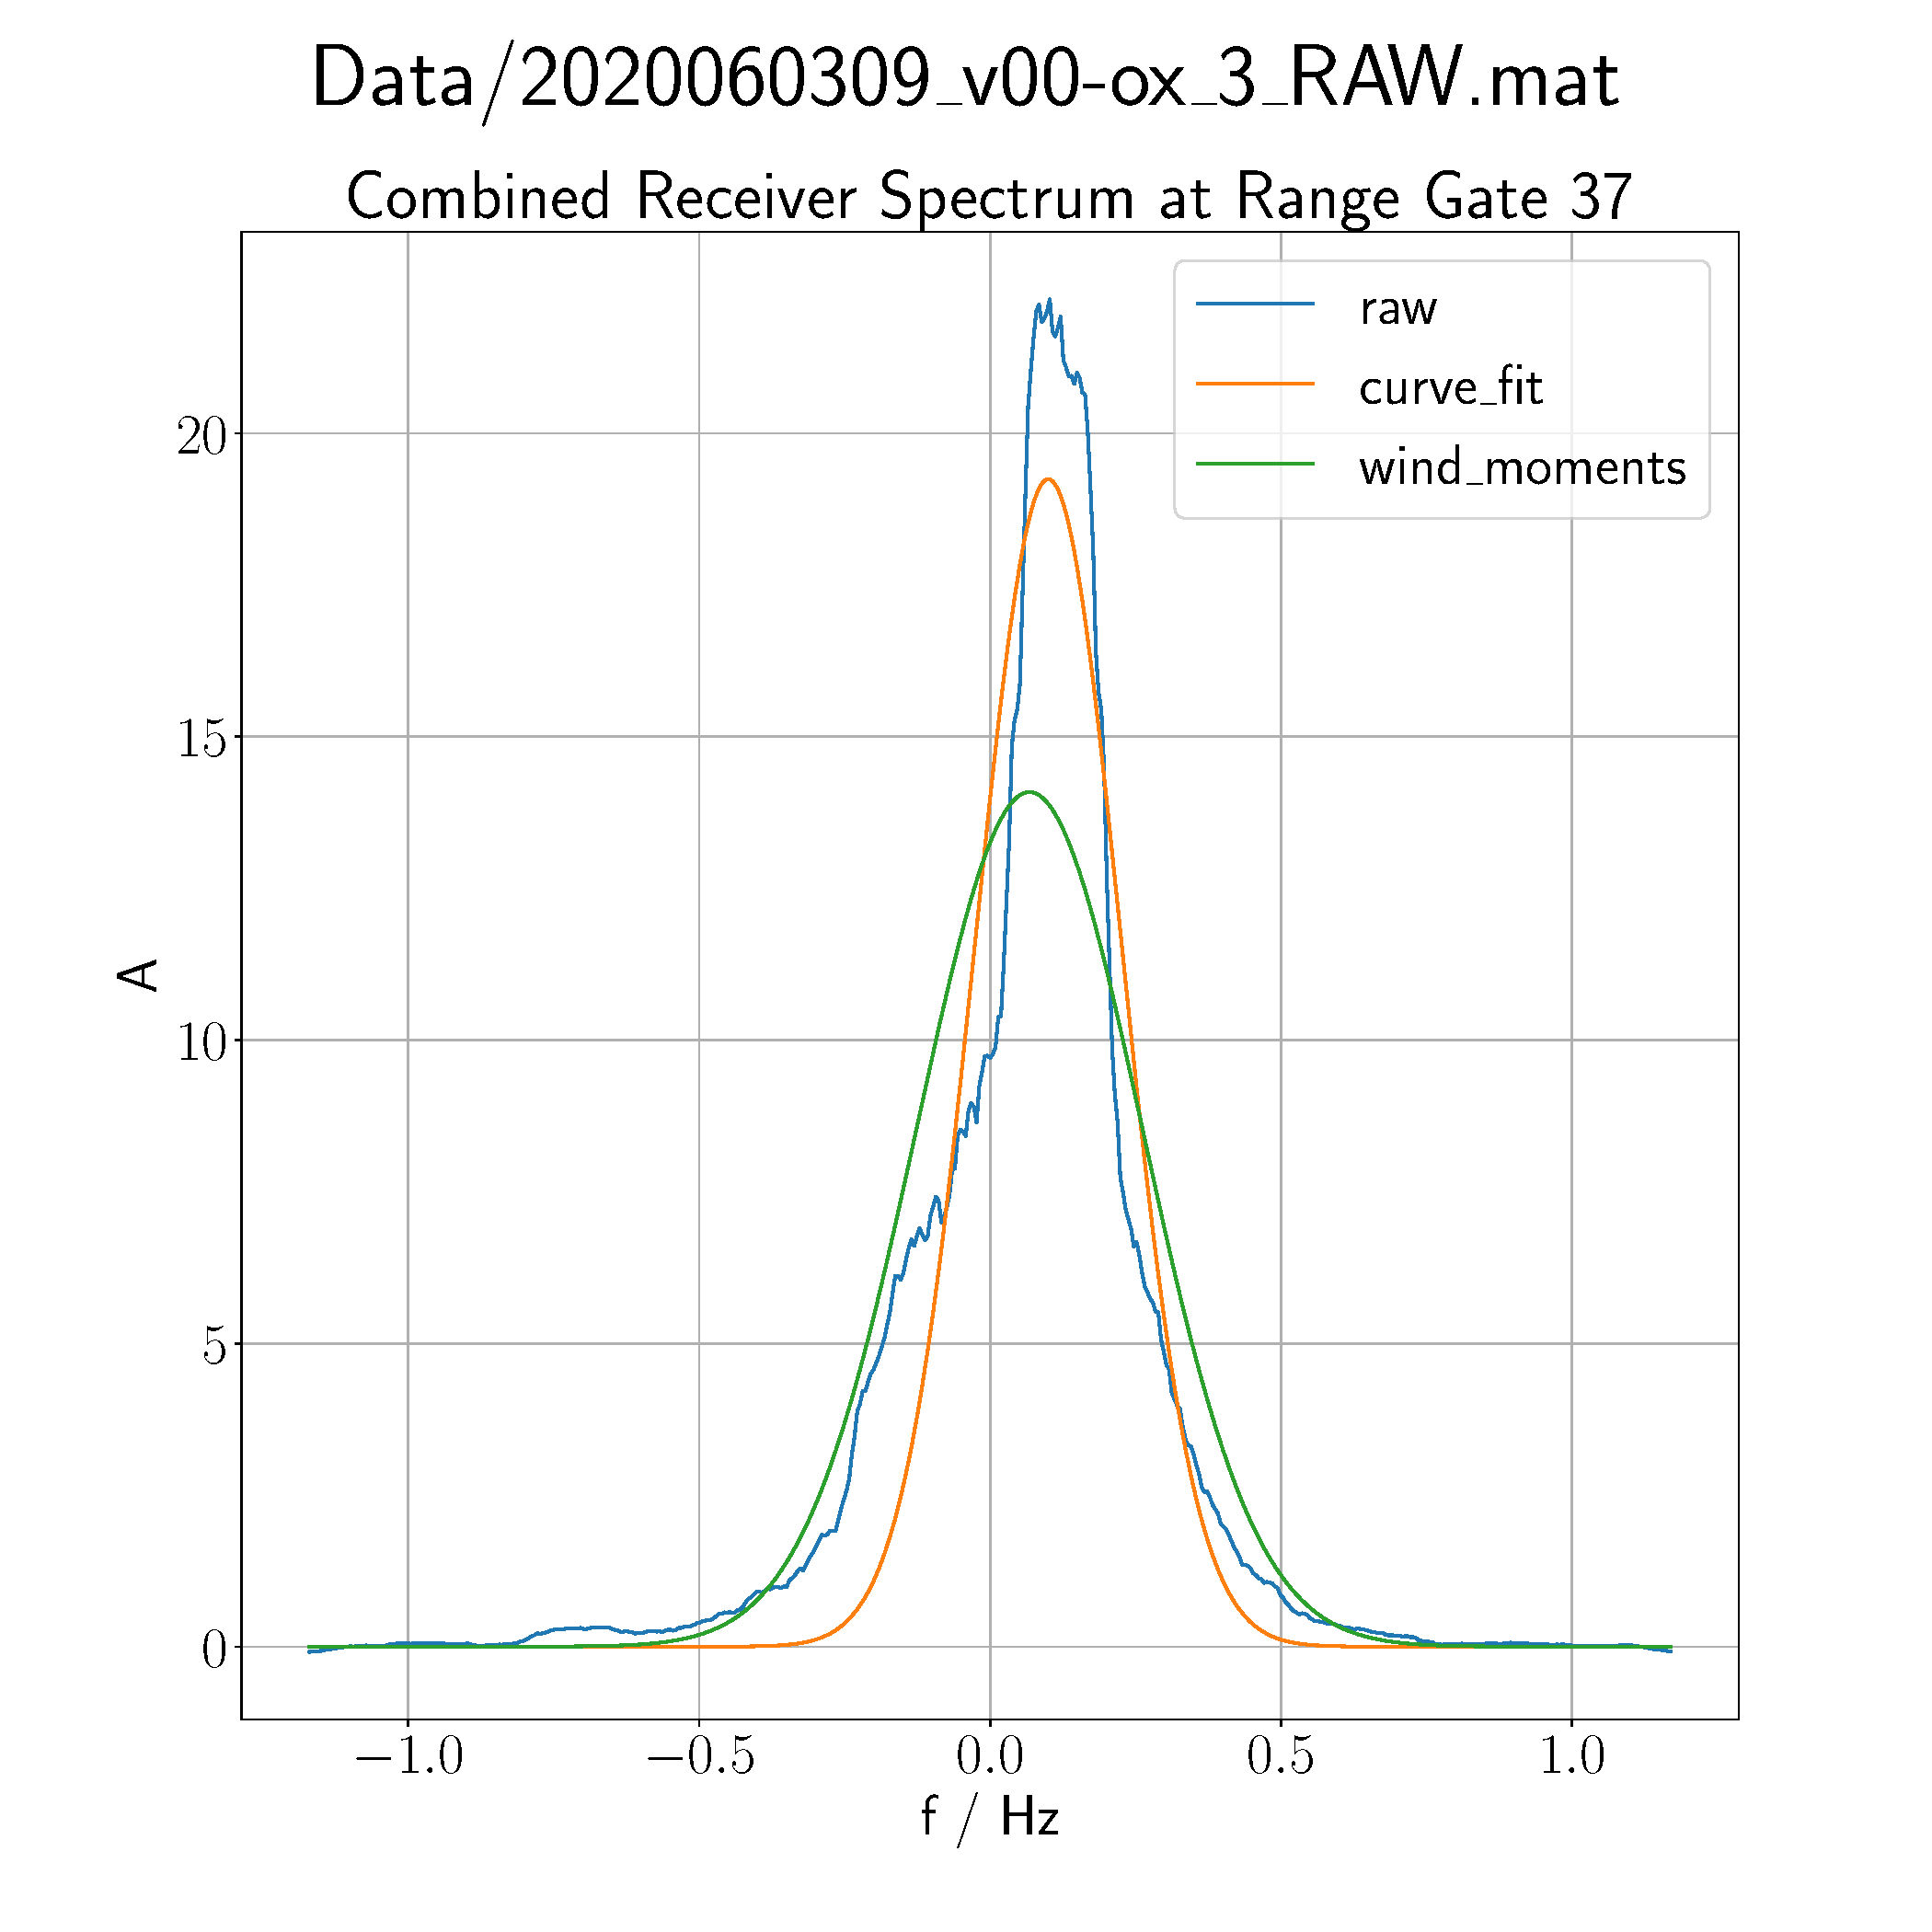
\includegraphics[width=\textwidth]{graphics/data_1_single_rg.pdf}
    \caption{}
  \end{minipage}\hfill
  \begin{minipage}[t]{0.45\textwidth}
    \centering
    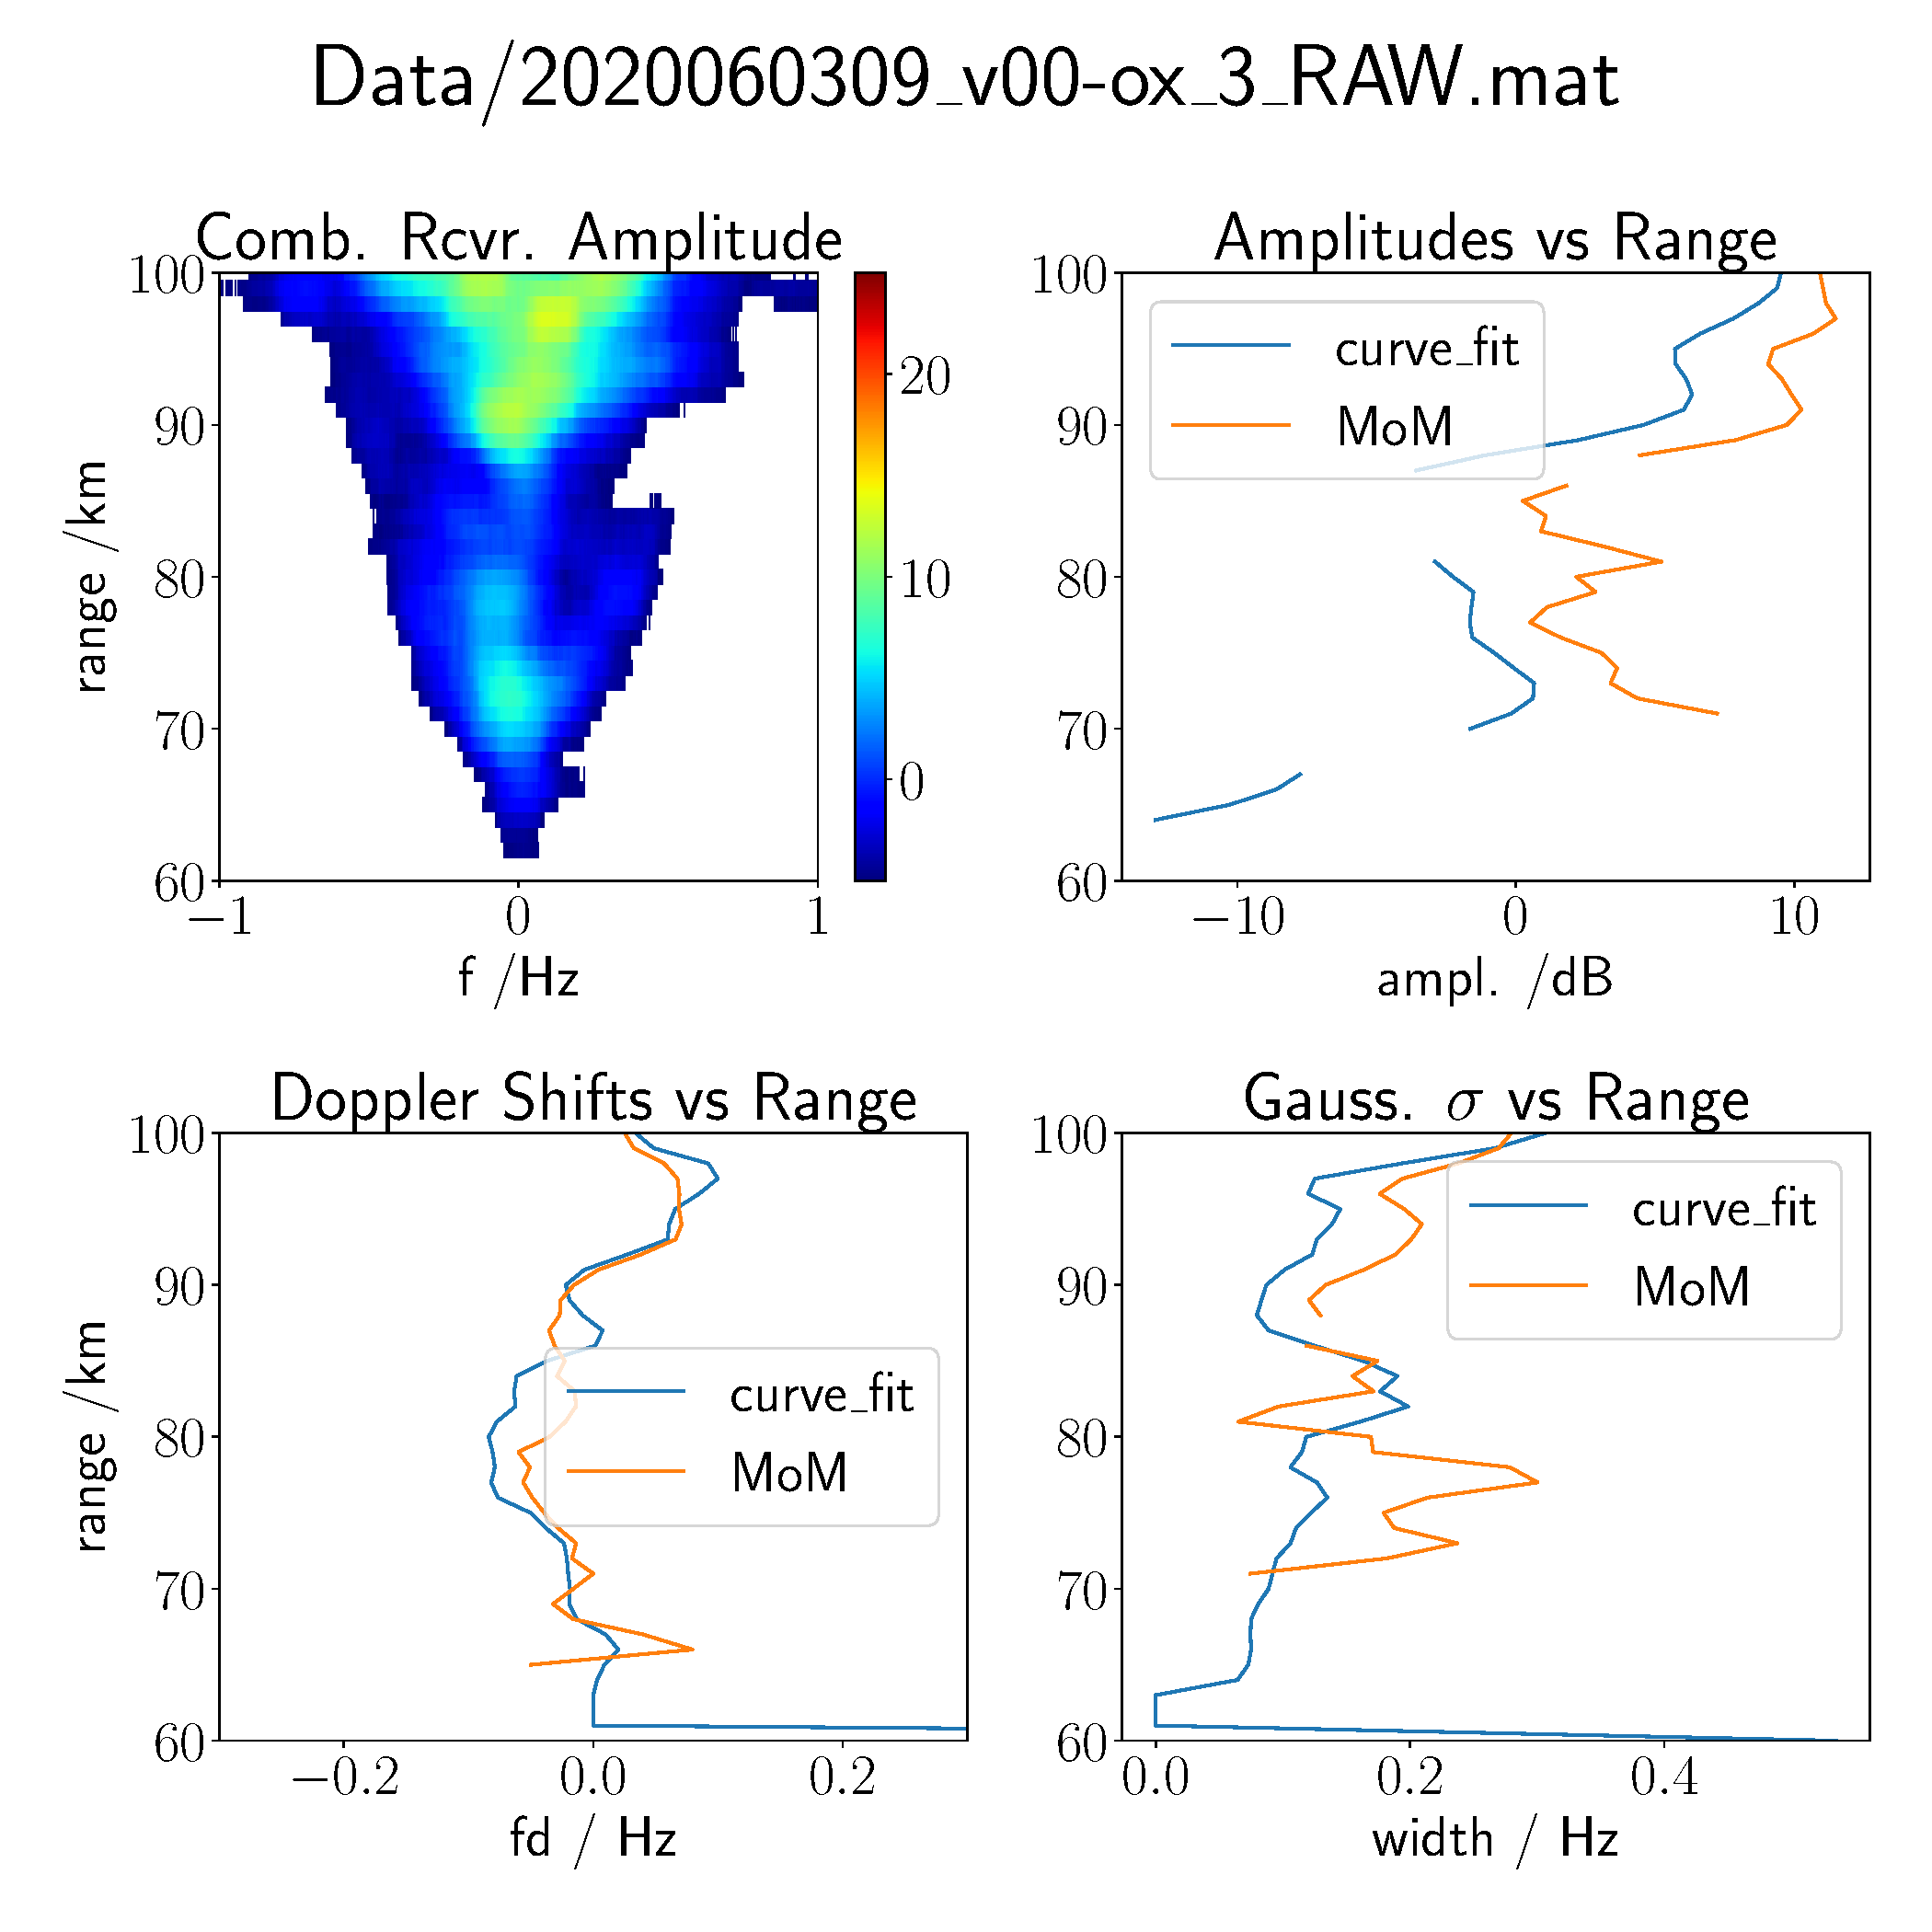
\includegraphics[width=\textwidth]{graphics/data_1_quad.pdf}
    \caption{}
   \end{minipage}
\end{figure}

\subsection{File 3}
\begin{figure}[H]
  \begin{minipage}[t]{0.45\textwidth}
    \centering
    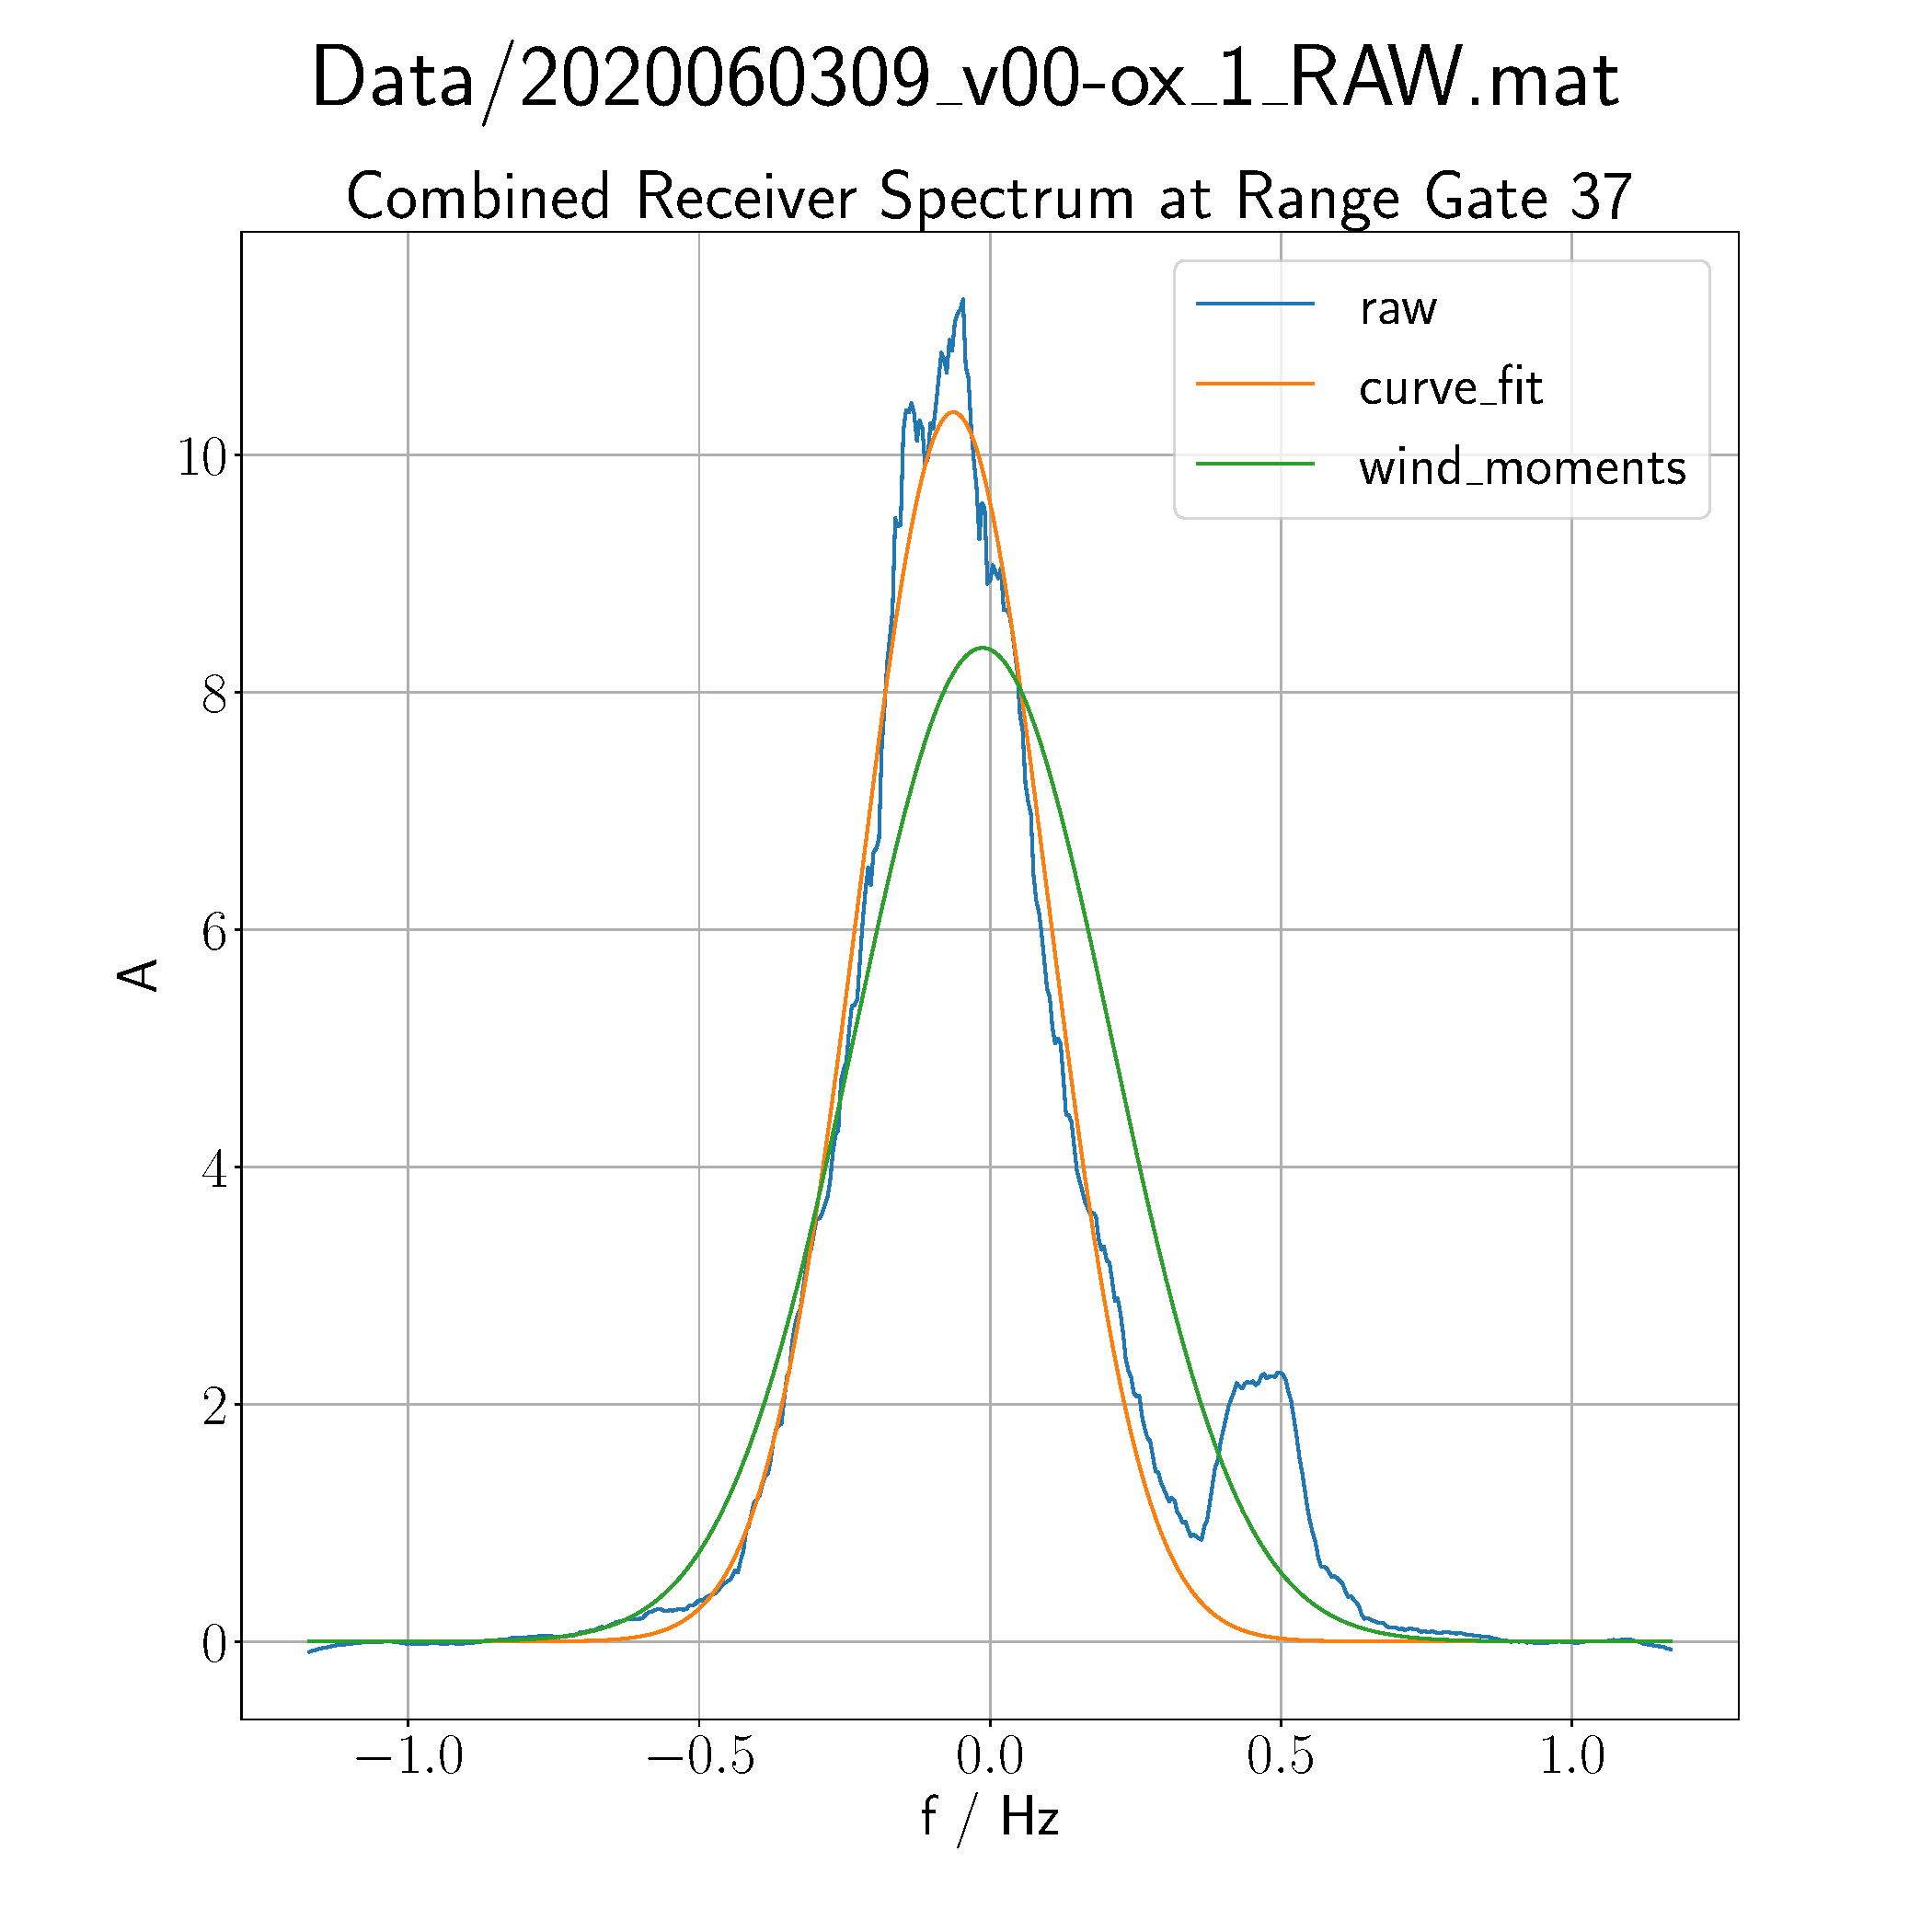
\includegraphics[width=\textwidth]{graphics/data_2_single_rg.pdf}
    \caption{}
  \end{minipage}\hfill
  \begin{minipage}[t]{0.45\textwidth}
    \centering
    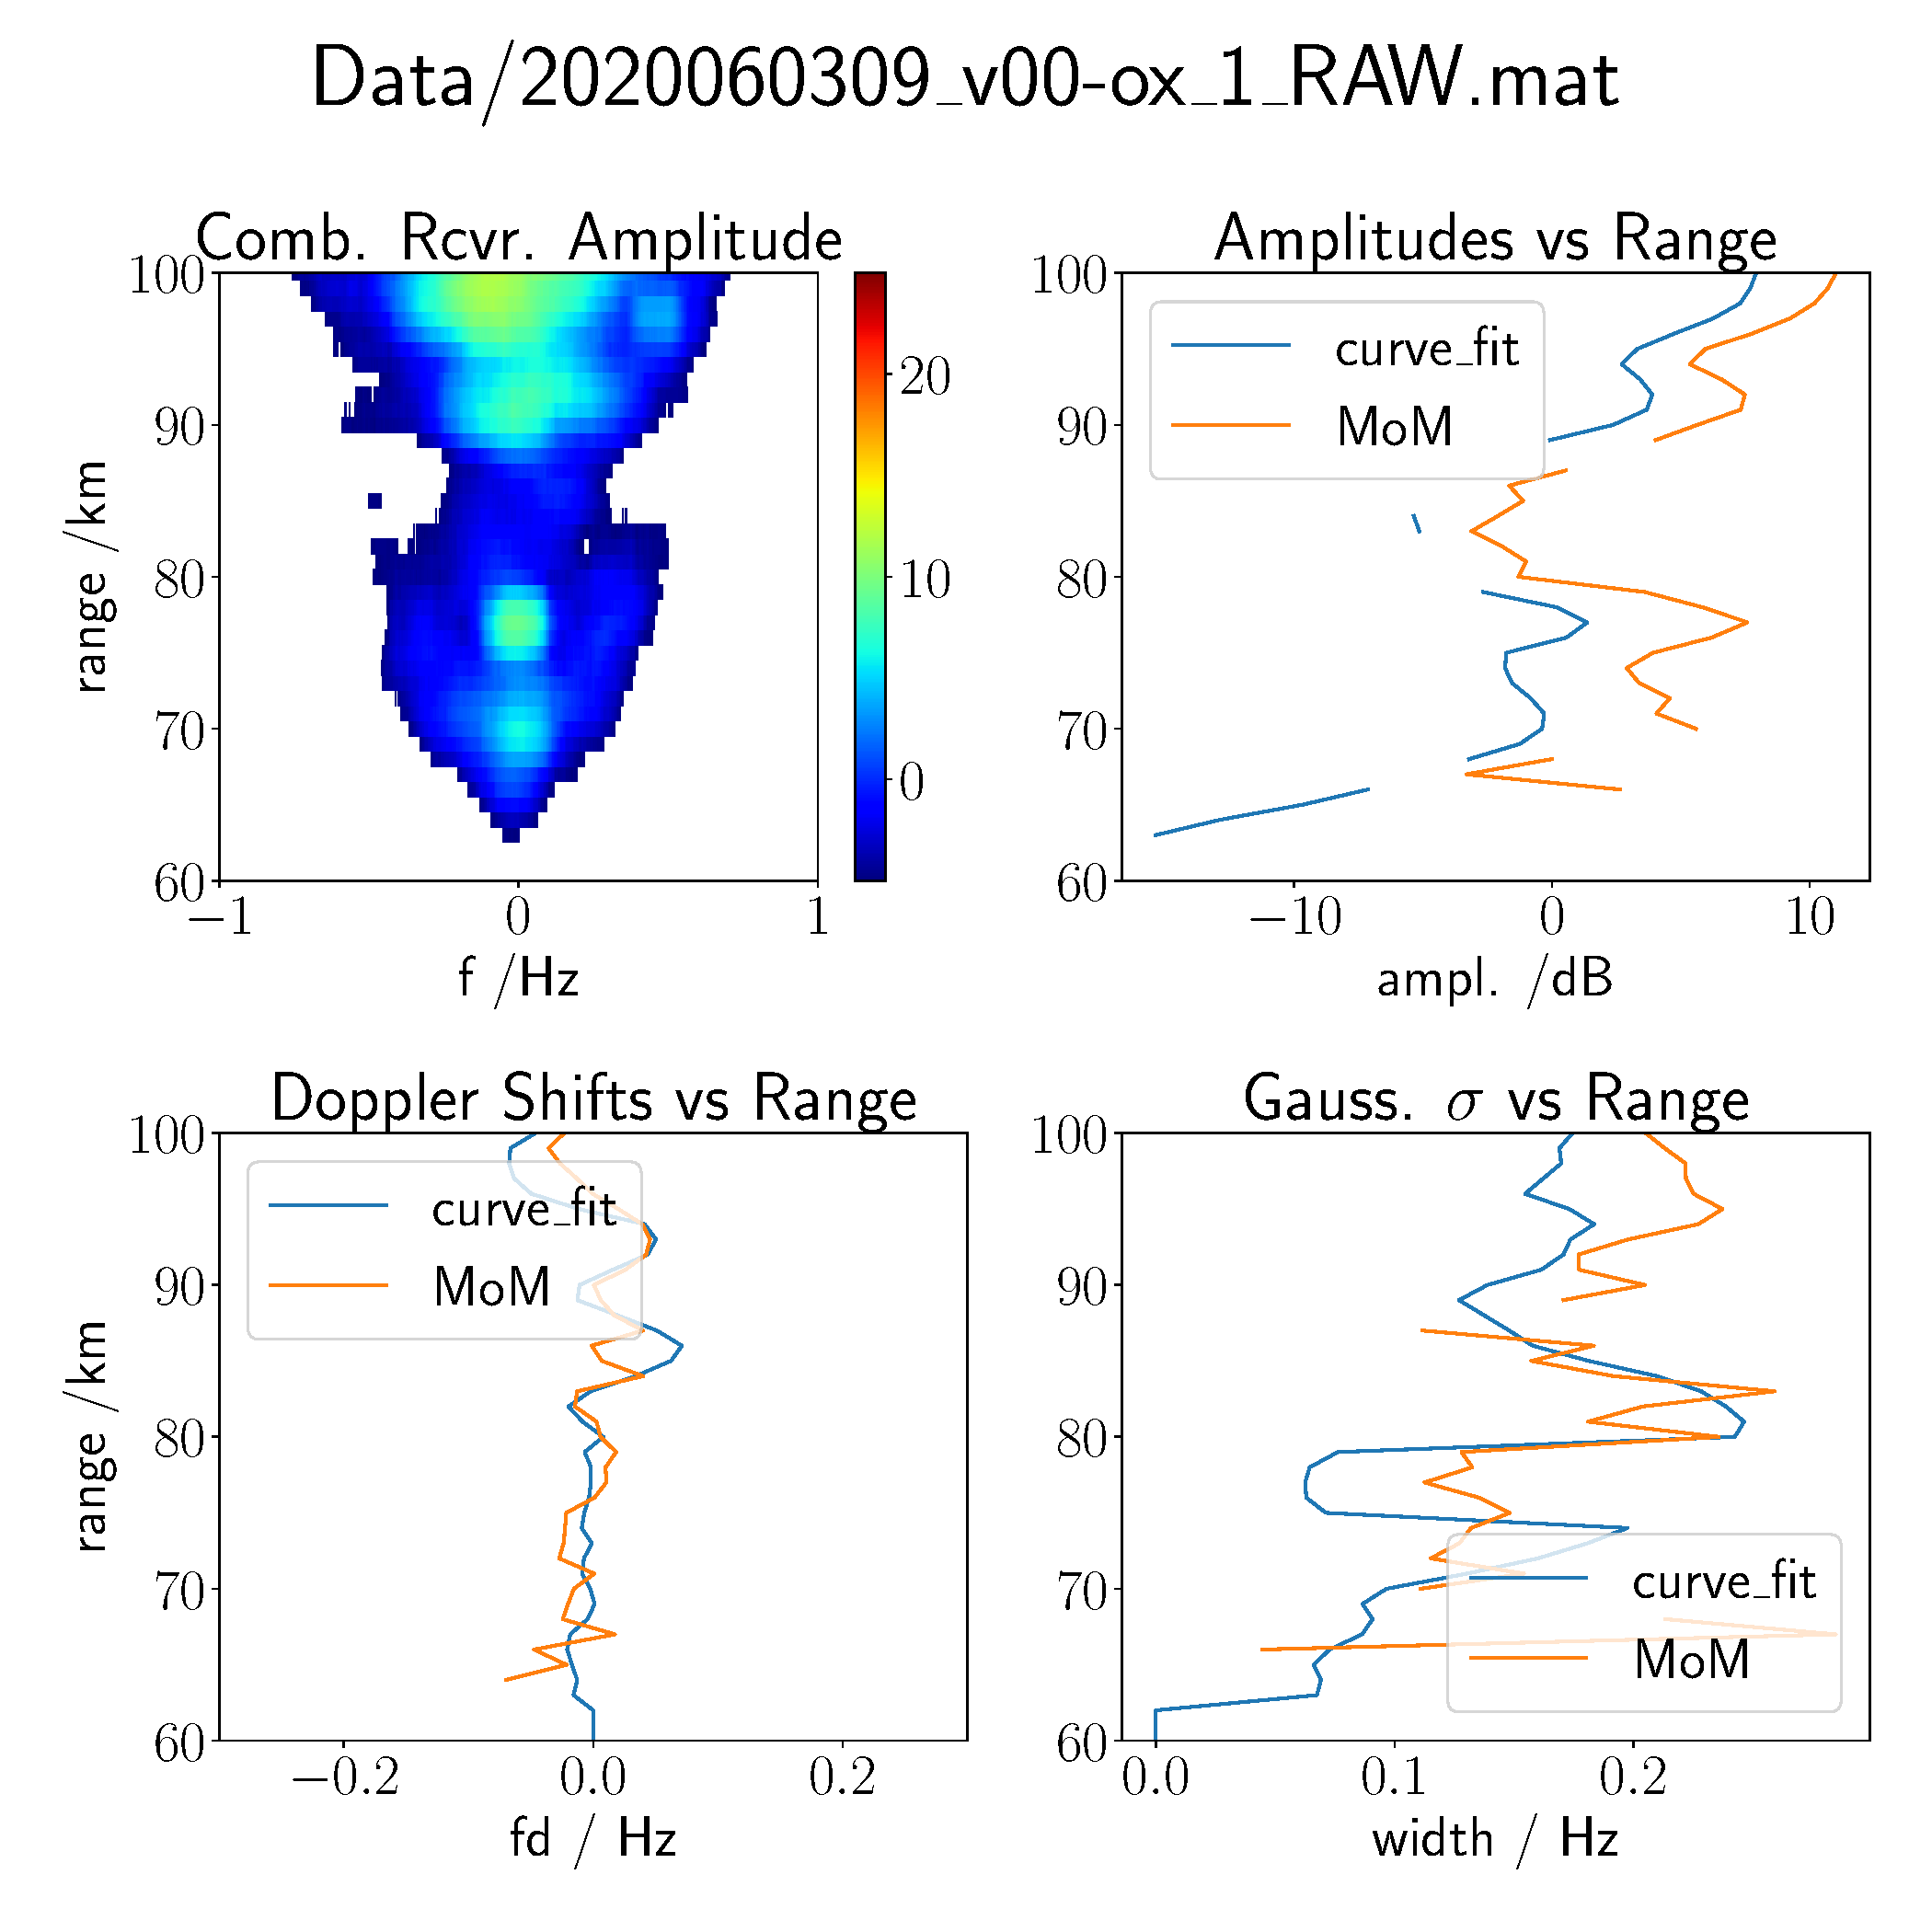
\includegraphics[width=\textwidth]{graphics/data_2_quad.pdf}
    \caption{}
   \end{minipage}
\end{figure}


\subsection{File 4}
\begin{figure}[H]
  \begin{minipage}[t]{0.45\textwidth}
    \centering
    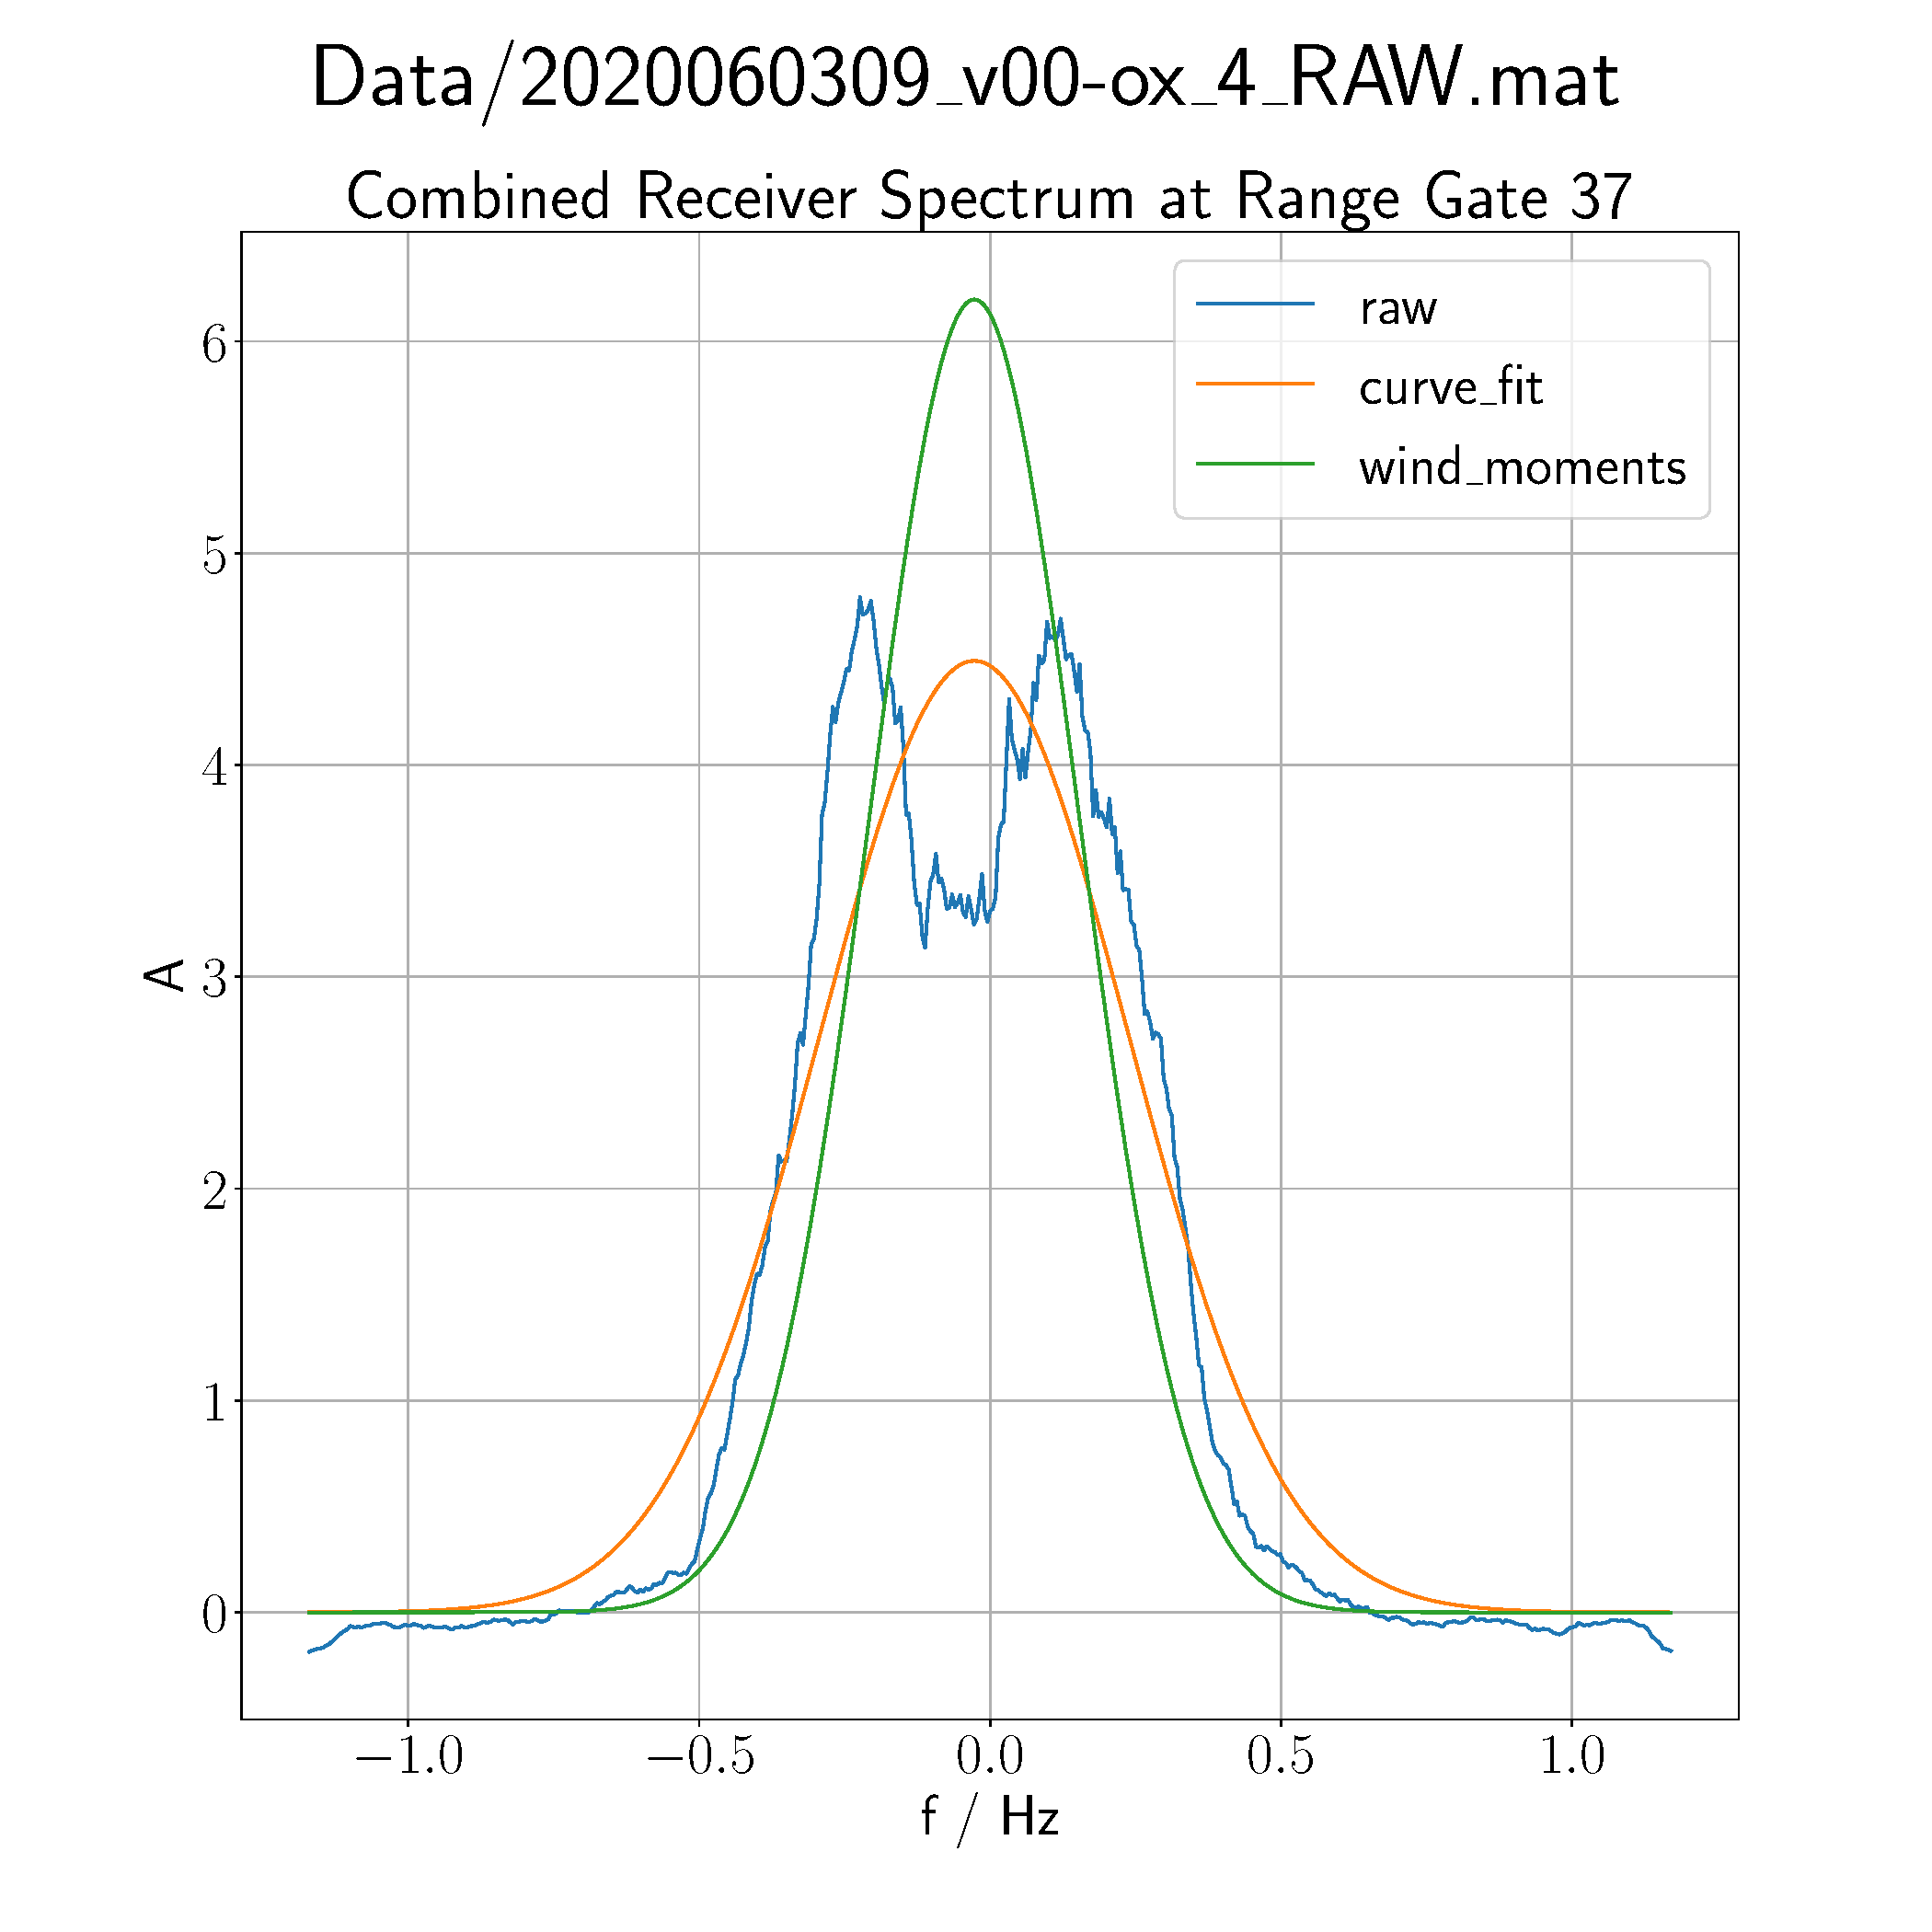
\includegraphics[width=\textwidth]{graphics/data_3_single_rg.pdf}
    \caption{}
  \end{minipage}\hfill
  \begin{minipage}[t]{0.45\textwidth}
    \centering
    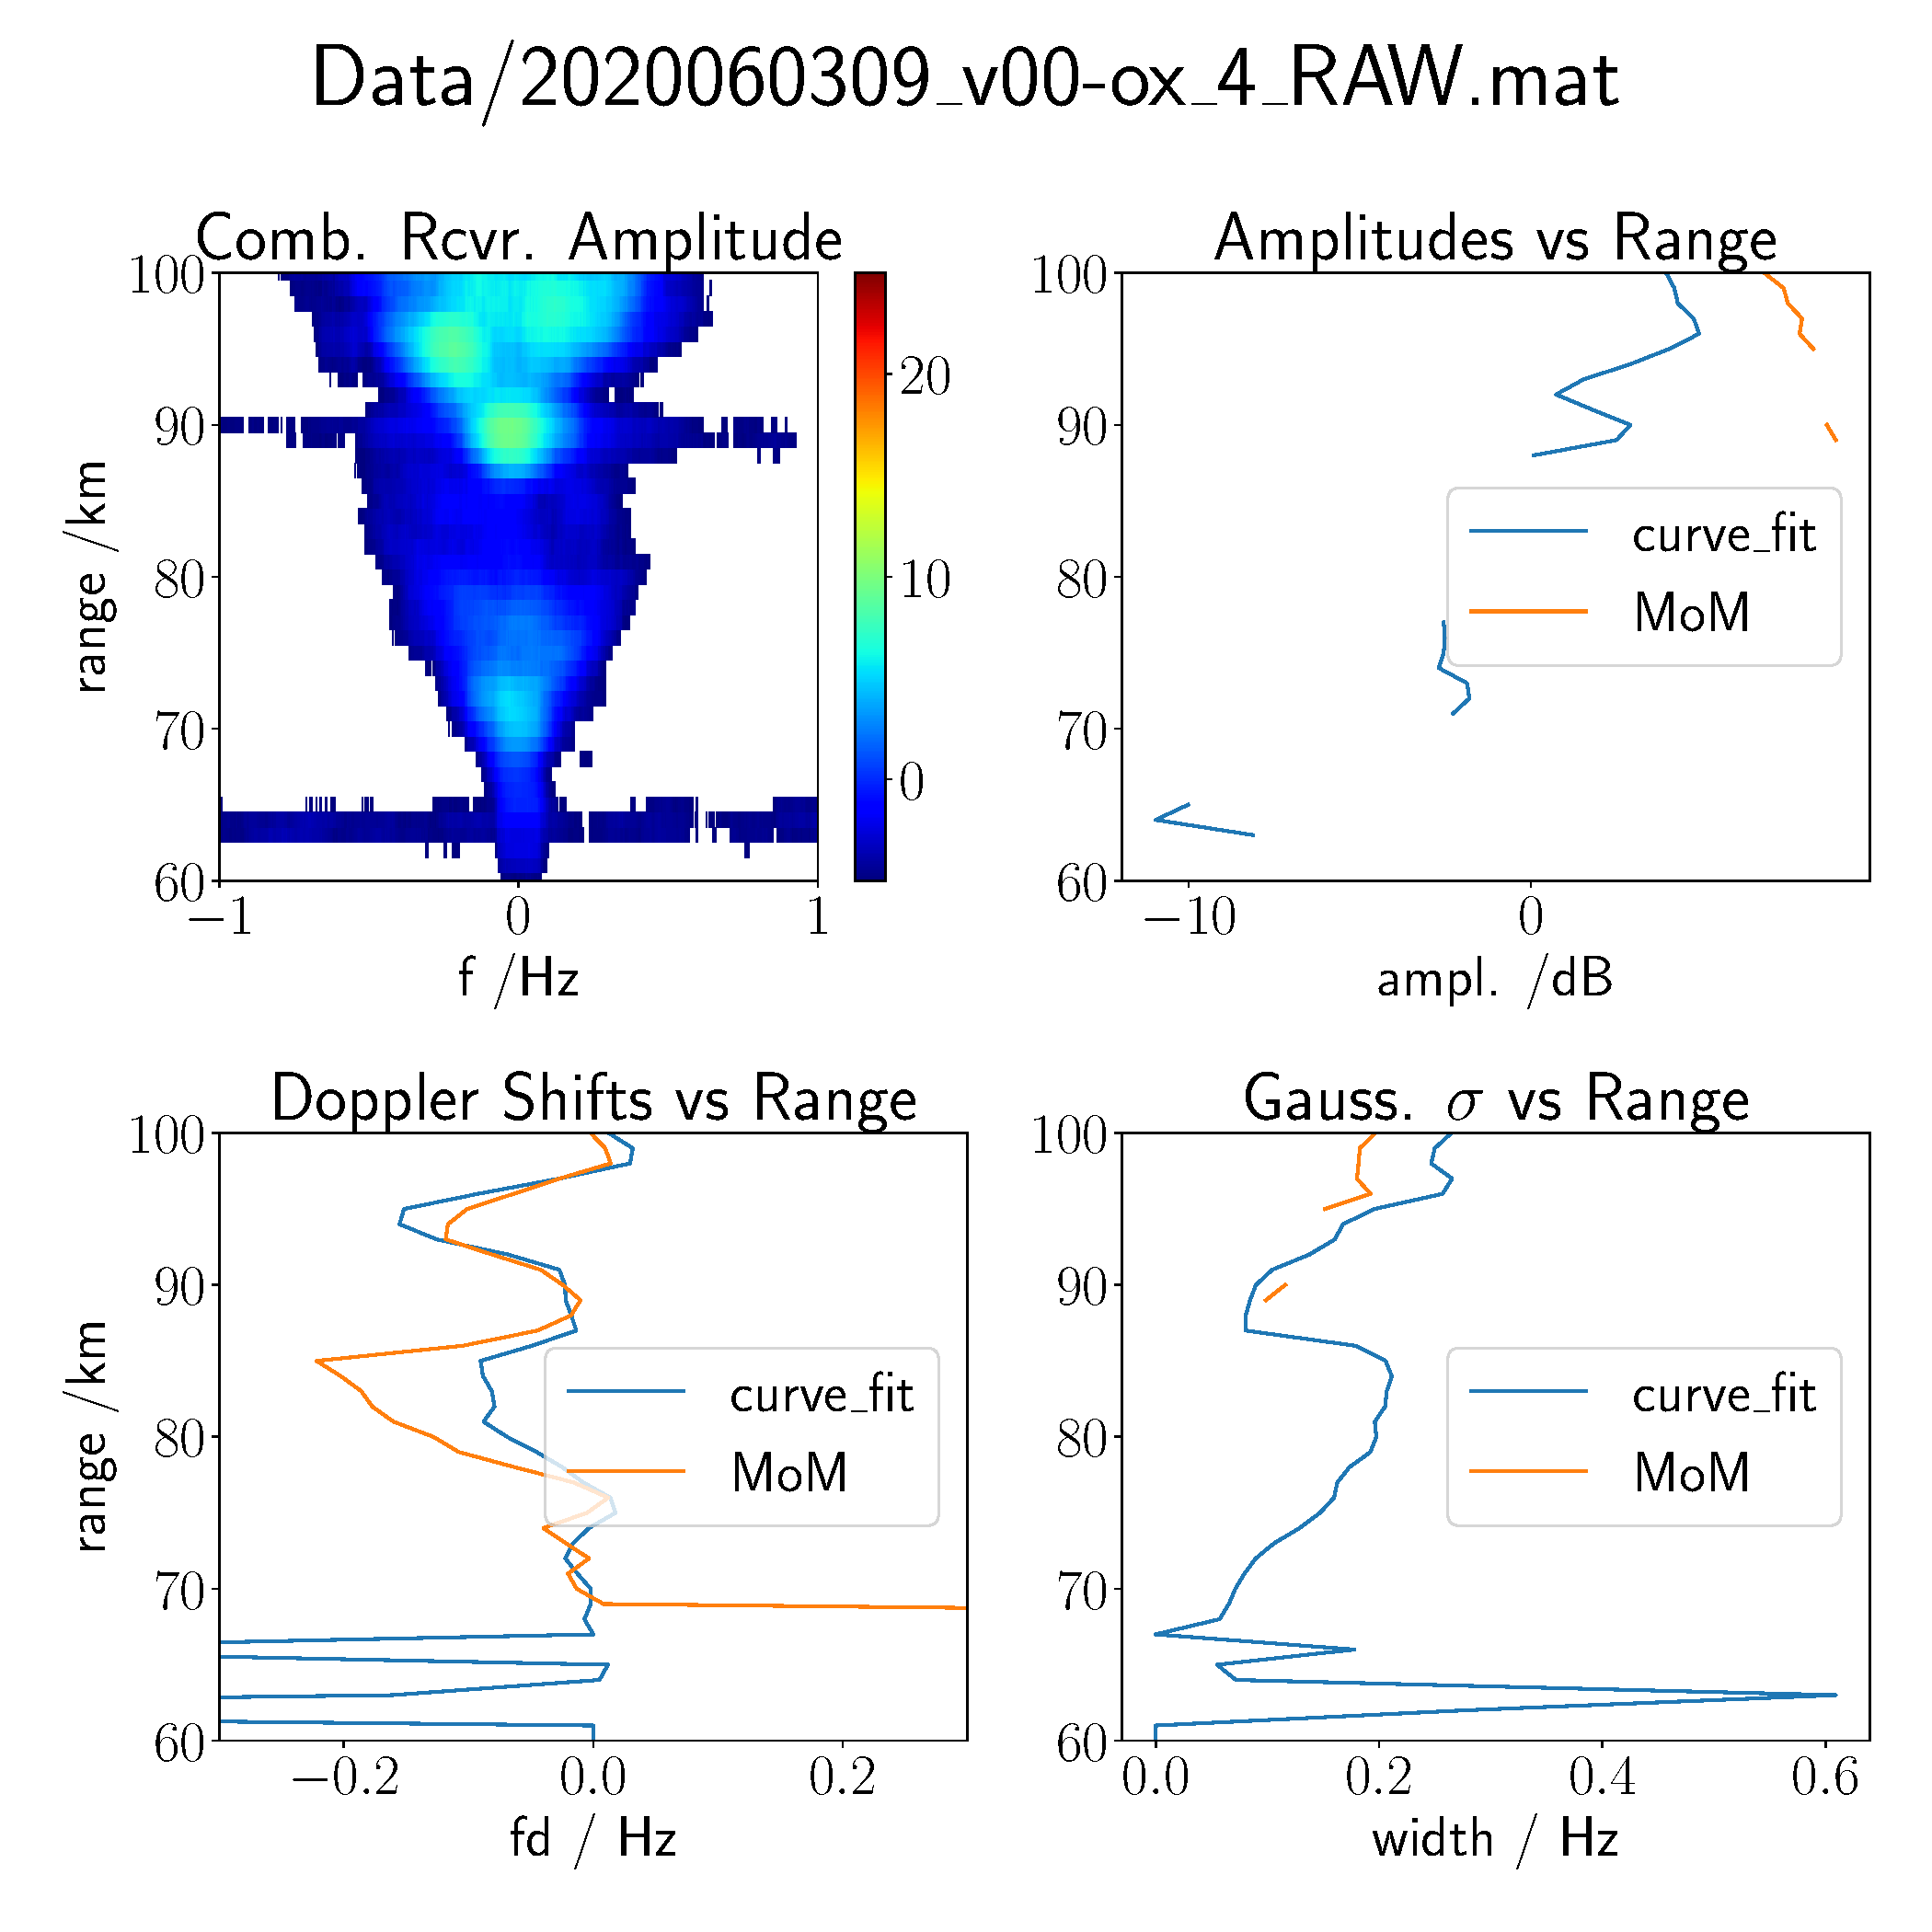
\includegraphics[width=\textwidth]{graphics/data_3_quad.pdf}
    \caption{}
   \end{minipage}
\end{figure}


\subsection{File 5}
\begin{figure}[H]
  \begin{minipage}[t]{0.45\textwidth}
    \centering
    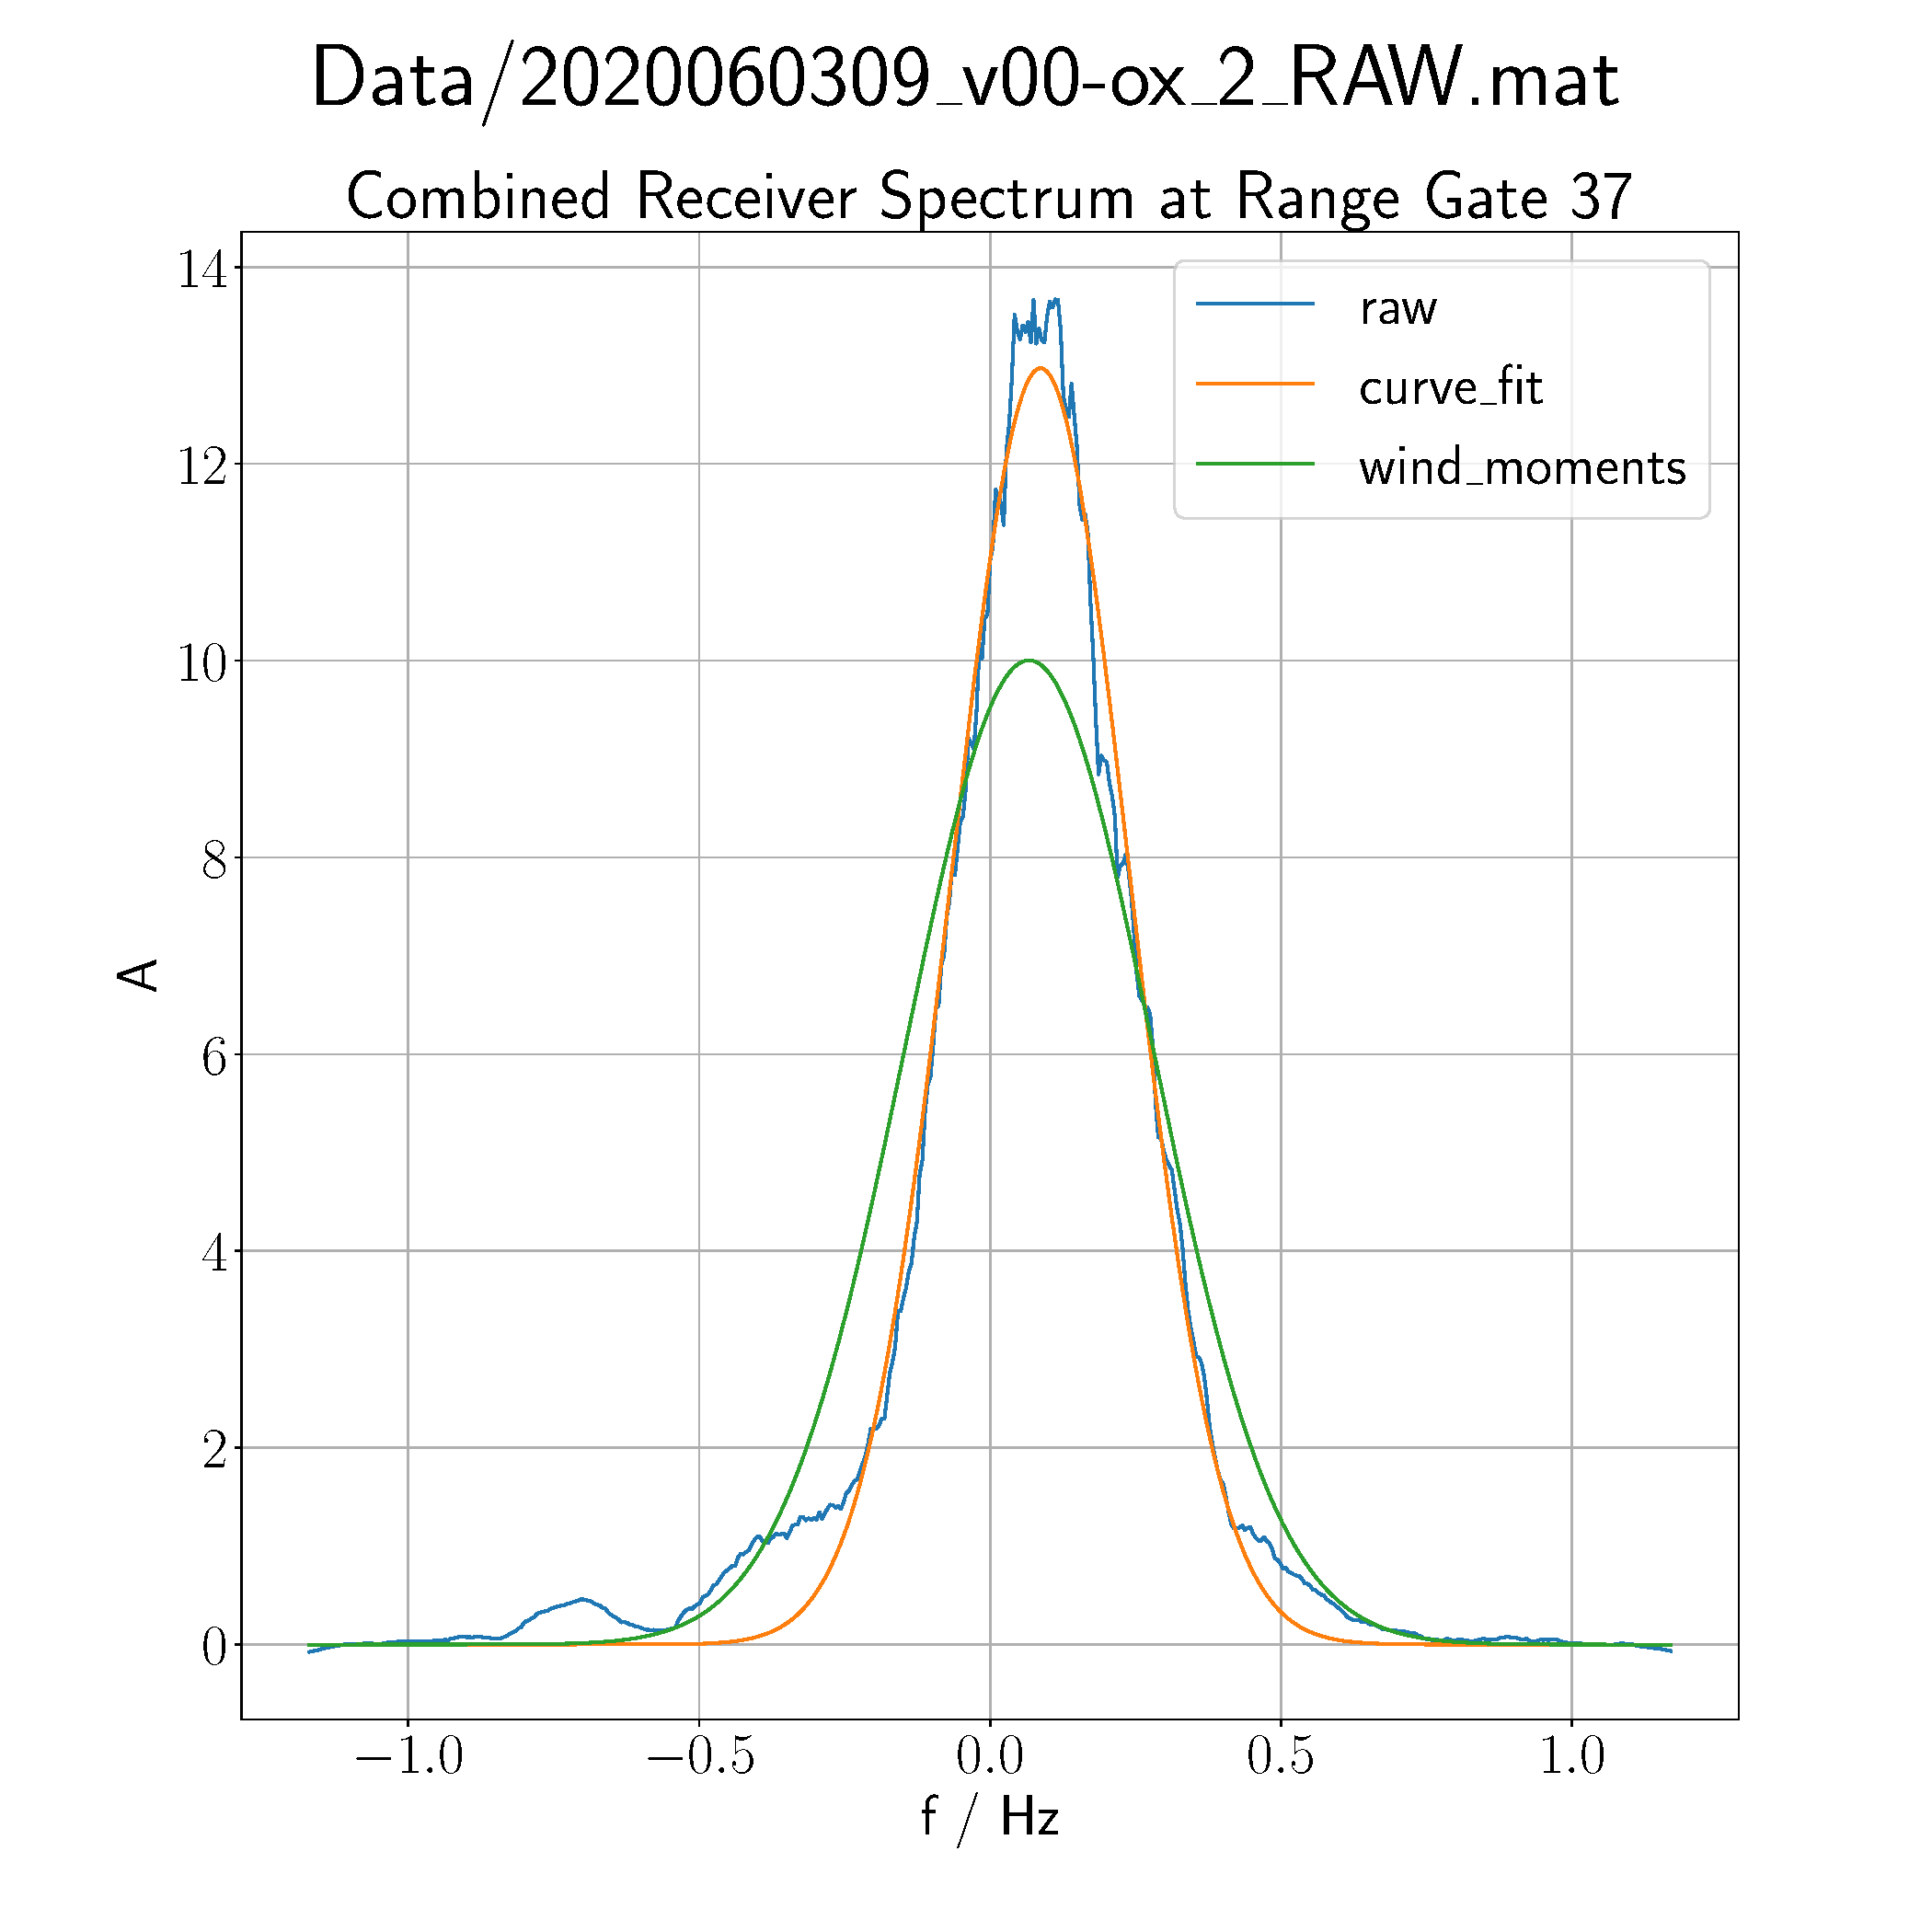
\includegraphics[width=\textwidth]{graphics/data_4_single_rg.pdf}
    \caption{}
  \end{minipage}\hfill
  \begin{minipage}[t]{0.45\textwidth}
    \centering
    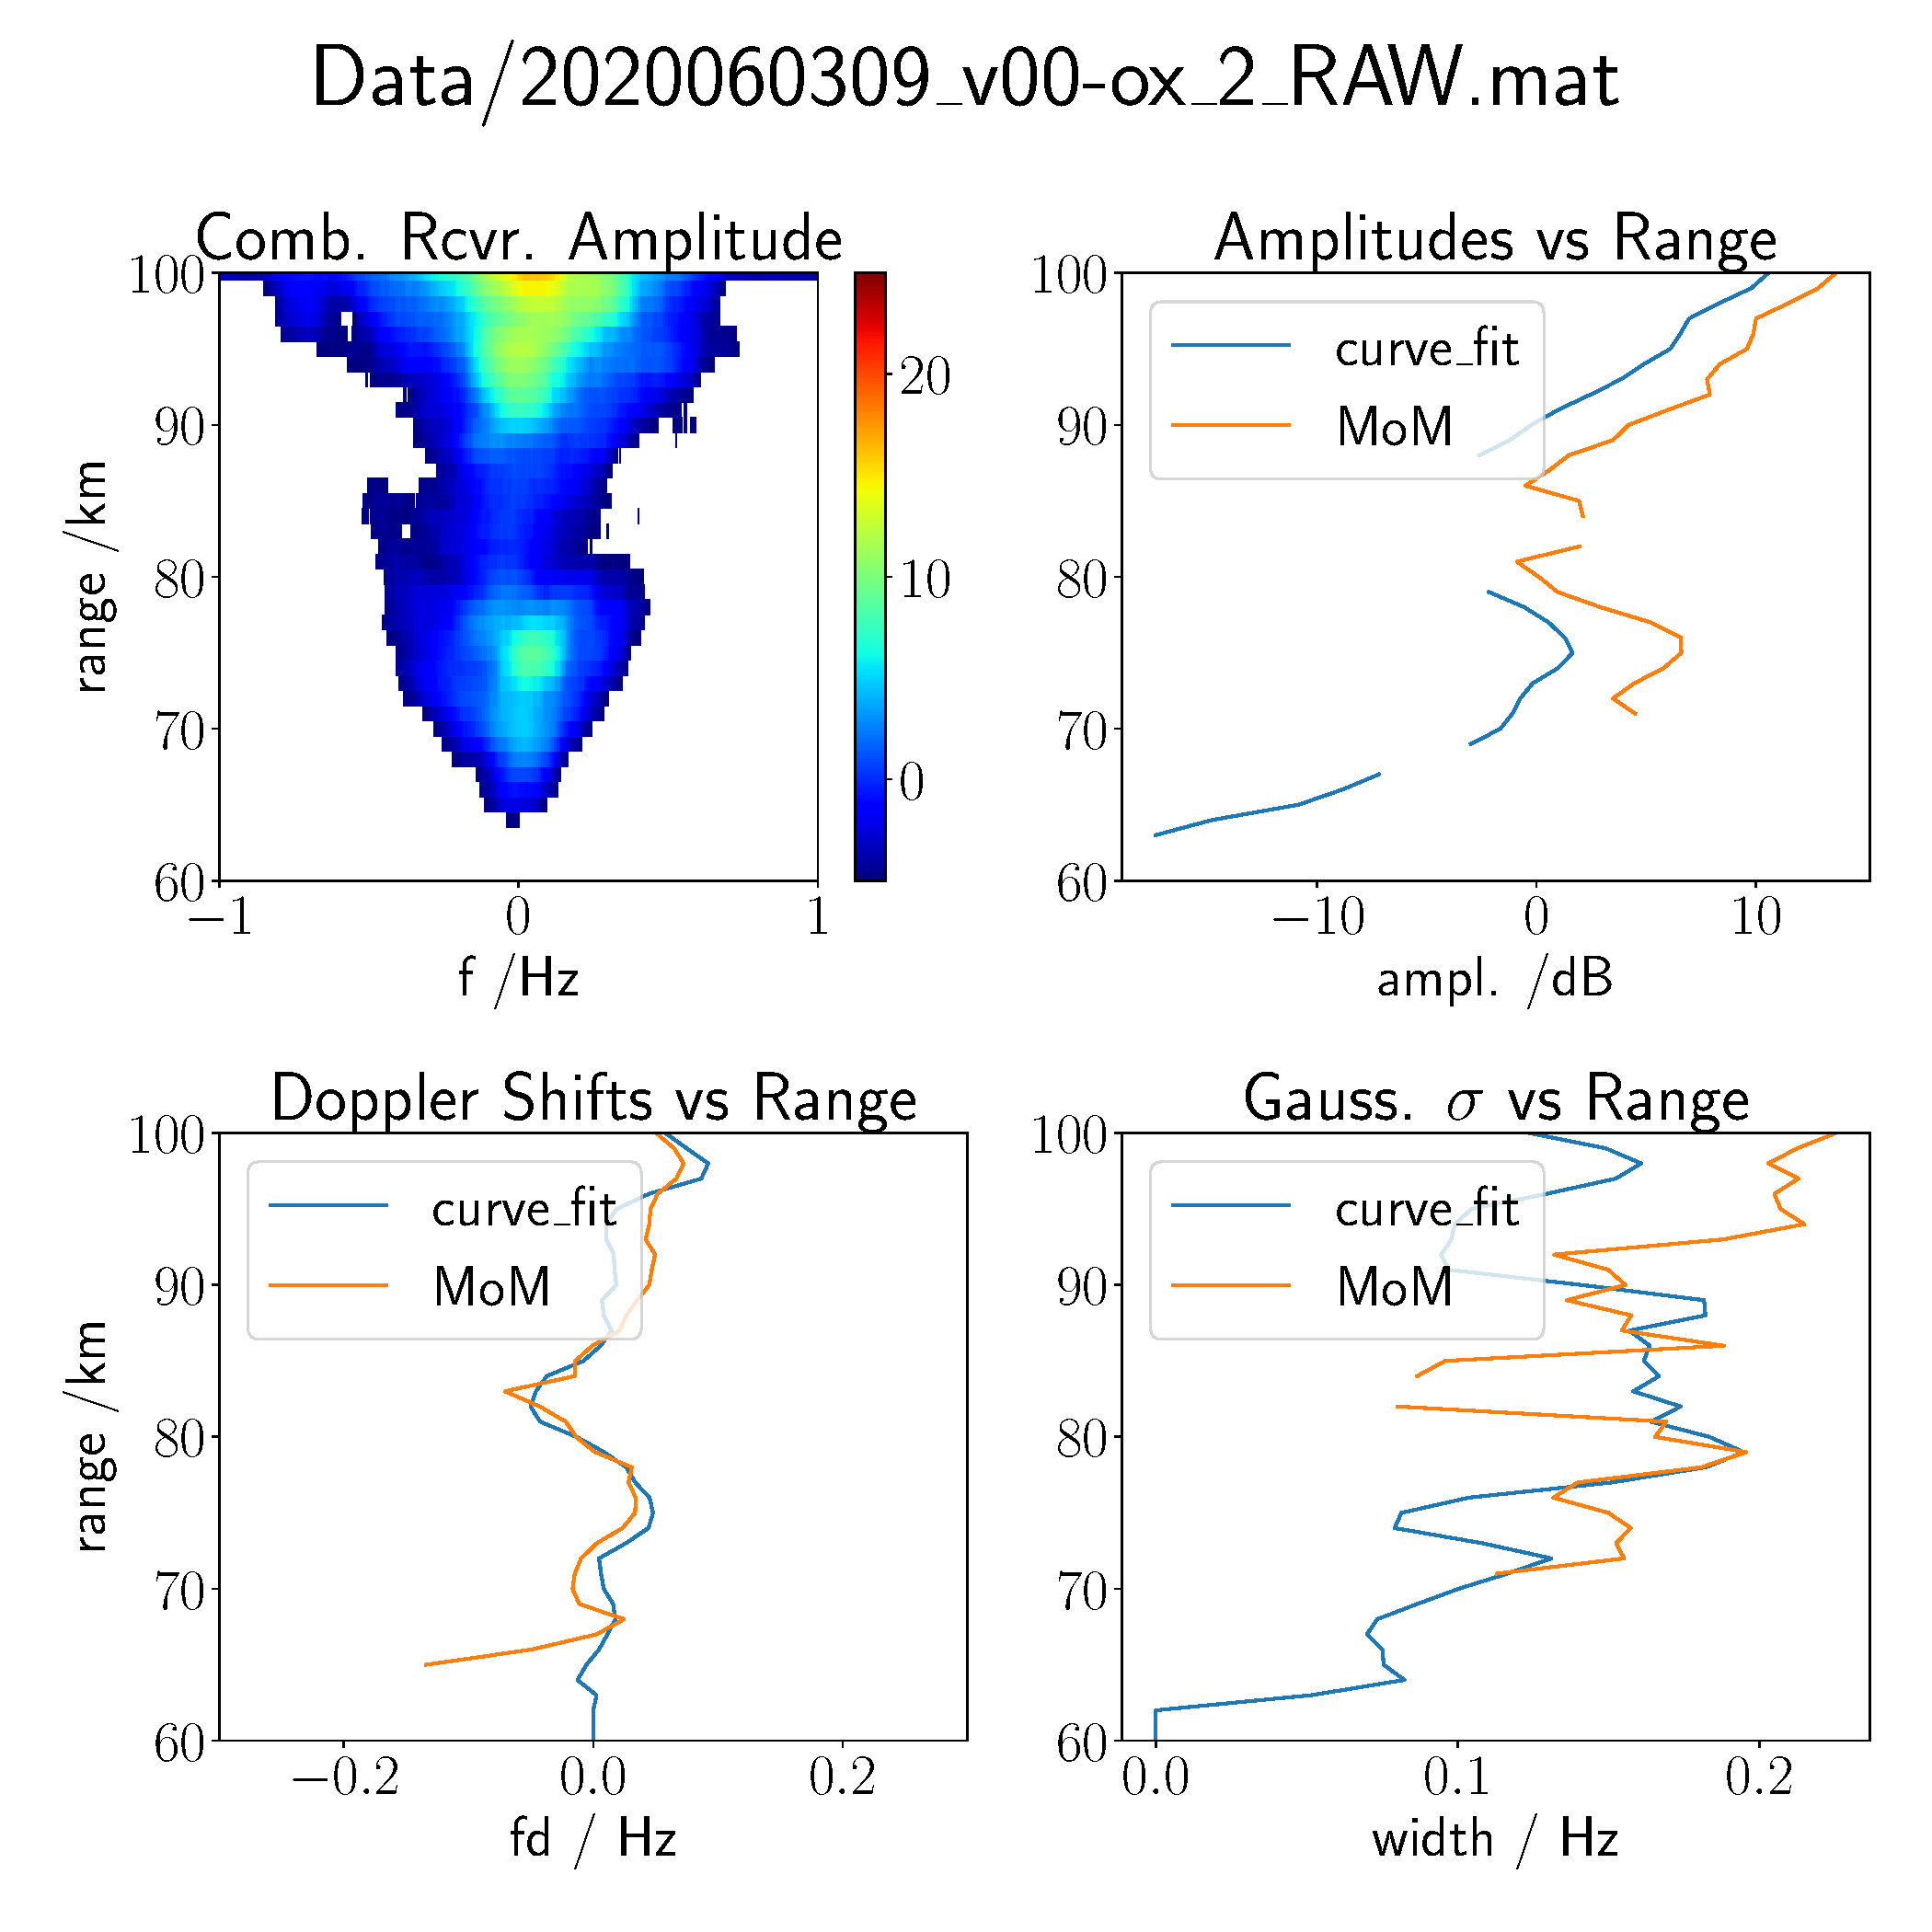
\includegraphics[width=\textwidth]{graphics/data_4_quad.pdf}
    \caption{}
   \end{minipage}
\end{figure}
